% ------------------------------Info--------------------------------
% Dieses Dokument ist als Vorlage f�r die studentischen Arbeiten
% am Institut f�r Thermodynamik gedacht. Es stellt eine einfache 
% M�glichkeit dar, die studentischen Arbeiten im Corporate Design
% der TU Braunschweig zu gestalten.
% Dazu wurden viele der notwendigen Einstellungen bereits in dieses
% Dokument eingearbeitet. Es steht dem Autor nat�rlich frei weitere
% Anpassungen, an seine individuellen kreativen Vorstellungen und 
% zum erfolgreichen Erstellen notwendigen Bed�rfnisse, vorzunehmen.
% Hierf�r sei an dieser Stelle auf die Website der Corporate Design
% (https://www.tu-braunschweig.de/presse/cd/toolbox) und die 
% Dokumentation zum Corporate Design in LaTeX hingewiesen.
%
% In diesem Sinne: Frohes Schreiben!
%-------------------------------------------------------------------

\documentclass[fontsize=11pt,
               paper=a4,	%Papierformat ist A4
               style=print, %[<print/printdev/screen>] Dokument ist f�r den Druck gedacht
               nexus, %Hausschrift der TU Braunschweig verwenden
               cmyk, % [<cmyk/rgb>]  Farben in CMYK Schema
               twoside=false, %Kein zweiseitiger Druck
               toc=bibliography ,%Literaturverzeichnis ohne Nummer im Inhaltsverzeichnis anzeigen
               blue % [<orange/blue/green/violet>] Farbschema f�r die Arbeit
              ]
              {tubsbook}
                       
%---------------------------------------------------
%---------------Allgemeine Angaben------------------
%---------------------------------------------------
\def \TITLE					{Adaptive Controller Design for Refrigeration Cycle Using the Natural Refrigerant  CO\textsubscript{2}}
\def \TYPE					{Masterarbeit} %[<Projektarbeit/Bachelorarbeit/Studienarbeit/Masterarbeit>]
\def \AUTHOR				{Julius Martensen}
\def \BETREUER				{Dipl. Ing. Michael N\"oding}
\def \TITELBILD				{pictures/Titelbild.png}
\def \AUFGABENSTELLUNG		{Aufgabenstellung.pdf}
\def \TOPLINE				{} %[<\showtopline>] % Aktiviert die rote Trennlinie �ber dem Bild. 
										%Sollte nur verwendet werden, wenn das Bild keine farbliche Trennung bietet.
%---------------------------------------------------
%----------Ende der Allgemeinen Angaben-------------
%
%		Header-Datei
%

% Nummerierungstiefe von section/subsection/subsubsection
\setcounter{secnumdepth}{3} 

%Absatzeinzug einstellen
\setlength{\parindent}{1em}
\setlength{\parskip}{0pt}

% Deutsche Rechtschreibung und deutscher Zeichensatz
\usepackage{german,ngerman}
\usepackage[ansinew]{inputenc}  

% Aktuelles Datum ermitteln
\usepackage[ngerman]{datenumber}

% Erweiterung f�r ein deutsches Literaturverzeichnis
\bibliographystyle{abbrvdin}

% Erweiterte Mathematikbibliotheken
\usepackage{amsmath}
\usepackage{amssymb}

% Ma�einhaeiten-Darstellung verbessern
\usepackage{units}

% Extra Symbole f�r die Verwendung im Text (z.B. \textcelsius)
%(werden nicht aus der Nexus-Schriftart einbunden)
\usepackage{textcomp}

% Einbinden von externen PDF Dateien
\usepackage[final]{pdfpages}

% Zum einbinden von Grafiken  
\usepackage{graphicx}
\usepackage{subcaption}  %erlaubt das erstellen von subfigures
\usepackage{float} %erm�glicht das erstellen von "non-floating figures"

%Hyperref f�r Verlinkungen im Dokument und URL's
%hyphens f�r verbesserten Zeilenumbruch in url's
\PassOptionsToPackage{hyphens}{url}
\usepackage[	breaklinks={true},
 						colorlinks	={true},
 					  	linkcolor	={tubsBlack},
  						citecolor	={tubsBlack},
  						filecolor	={tubsBlack},
  						urlcolor	={tuSecondaryMedium100},						
 					]{hyperref} %Interne Links in Schwarz und externe URL's in bg Farbe
 					
%Zus�tzliche Buchstaben und Zahlen erlauben f�r Zeilenumbruch bei url's (verbessert den Blocksatz)				
\expandafter\def\expandafter\UrlBreaks\expandafter{\UrlBreaks%  save the current one
  \do\a\do\b\do\c\do\d\do\e\do\f\do\g\do\i\do\j%
  \do\k\do\l\do\m\do\n\do\o\do\q\do\r\do\s%
  \do\u\do\v\do\w\do\x\do\y\do\z\do\A\do\B\do\C\do\D%
  \do\E\do\F\do\G\do\H\do\I\do\J\do\K\do\L\do\M\do\N%
  \do\O\do\P\do\Q\do\R\do\S\do\T\do\U\do\V\do\W\do\X%
  \do\Y\do\Z\do\1\do\2\do\3\do\4\do\5\do\6\do\7\do\8\do\9} 	
  
% R�ckseiten-Elemente
\address{% Addresse
  Technische Universit�t Braunschweig\\
  Institut f�r Thermodynamik\\
  Hans-Sommer-Strasse 5\\
  38106 Braunschweig}
\backpageinfo{}				

%Makro zur Formatierung des Anhangs
\newcommand{\Anhang}{
\appendix
\chapter*{Anhang}
\addcontentsline{toc}{chapter}{Anhang}
\setcounter{chapter}{1}
\markboth{Anhang}{Anhang}
\label{Anhang}}

%Makro zur Formatierung von der Titelseite bis zum Inhaltsverzeichniss
\newcommand{\Anfang}{
\pagenumbering{Roman}
\begin{titlepage}
%Designhelper f�r Erstellung 
%\showdesignhelper

\showtubslogo[right]
\showlogo{
\includegraphics{ift_4C.pdf}}
\TOPLINE

%Titelbild f�r die Arbeit
\begin{titlerow}[bgimage=\TITELBILD ,imagefit=cropped]{3}


\hfill\vfill
\end{titlerow}
\begin{titlerow}[bgcolor=tuSecondaryDark100, c]{2}

\begin{fitbox}{\textwidth}{100pt}
\raggedright
\color{tubsWhite}
\textbf{\TITLE}
\end{fitbox}
\addvspace{1,5em}
\begin{Large}
\raggedright
\color{tubsWhite}
\textbf{\TYPE}\vfill
\end{Large}

\end{titlerow}
\begin{titlerow}[bgcolor=tuSecondaryMedium80]{3}
\color{tubsWhite}


\begin{tabbing}
\hspace*{2.0cm}   \=  \hspace*{12.0cm}        \= \kill
\textbf{Autor:} \> \textbf{\AUTHOR} \\
\textbf{Betreuer:} \> \textbf{\BETREUER}\\
\textbf{Pr\"ufer:} \> \textbf{Prof. Dr.-Ing. J\"urgen K\"ohler}\\


 \> \textbf{\today}
\end{tabbing}
\hfill\vfill
\end{titlerow}
\hfill\vfill
\end{titlepage}

\includepdf[pages=-]{\AUFGABENSTELLUNG}
\addchap*{Eidesstattliche Erkl�rung}


\vspace*{5cm}


Hiermit erkl�re ich eidesstattlich, dass ich diese Arbeit eigenst�ndig angefertigt und keine anderen als die angegebenen Hilfsmittel verwendet habe.
\vspace{3cm}\\
Braunschweig den \today
\tableofcontents
\pagenumbering{arabic}
\setcounter{page}{1}}



%Makro zum einpassen des Titels in die Titelbox
\usepackage{environ}
\newdimen\fontdim
\newdimen\upperfontdim
\newdimen\lowerfontdim
\newif\ifmoreiterations
\fontdim12pt
\makeatletter
\NewEnviron{fitbox}[2]{% \begin{fitbox}{<width>}{<height>} stuff \end{fitbox}
  \def\buildbox{%
    \setbox0\vbox{\hbox{\minipage{#1}%
      \fontsize{\fontdim}{1.2\fontdim}%
      \selectfont%
      \stuff%
    \endminipage}}%
    \dimen@\ht0
    \advance\dimen@\dp0
  }
  \def\stuff{\BODY}% Store environment body
  \buildbox
  % Compute upper and lower bounds
  \ifdim\dimen@>#2
    \loop
      \fontdim.5\fontdim % Reduce font size by half
      \buildbox
    \ifdim\dimen@>#2 \repeat
    \lowerfontdim\fontdim
    \upperfontdim2\fontdim
    \fontdim1.5\fontdim
  \else
    \loop
      \fontdim2\fontdim % Double font size
      \buildbox
    \ifdim\dimen@<#2 \repeat
    \upperfontdim\fontdim
    \lowerfontdim.5\fontdim
    \fontdim.75\fontdim
  \fi
  % Now try to find the optimum size
  \loop
    %\message{Bounds: \the\lowerfontdim\space
    %         \the\fontdim\space \the\upperfontdim^^J}
    \buildbox
    \ifdim\dimen@>#2
      \moreiterationstrue
      \upperfontdim\fontdim
      \advance\fontdim\lowerfontdim
      \fontdim.5\fontdim
    \else
      \advance\dimen@-#2
      \ifdim\dimen@<10pt
        \lowerfontdim\fontdim
        \advance\fontdim\upperfontdim
        \fontdim.5\fontdim
        \dimen@\upperfontdim
        \advance\dimen@-\lowerfontdim
        \ifdim\dimen@<.2pt
          \moreiterationsfalse
        \else
          \moreiterationstrue
        \fi
      \else
        \moreiterationsfalse
      \fi
    \fi
  \ifmoreiterations \repeat
  \box0% Typeset content
}
\makeatother %Header zum Einbinden der Packages und zur Layout formatierung/konfiguration
\begin{document}
\Anfang

%---------------------------------------------------
%--------------Beginn eigener Kapitel---------------
%---------------------------------------------------
\chapter{Introduction}\label{c:intro}

\section{Motivation}\label{c:intro:s:motivation}

The great motivational Speak follows in this section.

Hier schon folgende Quellen erwähnen:

\cite{Astrom1973}

\section{Literature Review}\label{c:intro:s:literature}

The great literature review follows in this section.
%!TEX root = ../studentischeArbeiten.tex
\chapter{Thermodynamic Statement of the Problem}\label{c:thermo}

The following chapter gives a brief introduction to the needed basics from a thermodynamic point of view.\\

In the first section the system is described from a technical perspective followed by  a general thermodynamic process model. \\

Afterwards the model used for simulating the system in Dymola is explained. \\

At last the problem motivating this thesis is formulated in the context of thermodynamics.

\section{Process Description} \label{c:thermo:s:process}

\section{Problem Statement} \label{c:thermo:problem}
The aim of enginnering thermodynamics is - as stated earlier in Chap. \ref{c:intro} - to understand and optimize the  behaviour of technical systems used for energy transformation and transportation. Hence, a connection to the field of optimal control is a logical extension to maximize the efficiency. As described in sec. \ref{c:thermo:s:process} the systems states are general interconnected by both physical components and physical phenomena. In the following section the coupling due to physical phenomena will be investigated.\\

The process can be divided in three basic processes:
\begin{itemize}
\item Isobaric process with heat supply
\item Adiabatic isenthalpic process 
\item Isentropic process with exchange of (mechanical) work
\end{itemize}
We can characterize these processes using the First Law of Thermodynamics in differential form, see e.g. \cite[p.25]{Weigand2013}:

\begin{align}
\begin{split}
du &= d \left( h - pv \right ) \\ &= dh - v dp - p dv \\
&= \delta q + \delta w_{diss} - p dv
\end{split}
\label{c:thermo:e:firstlaw}
\end{align}
\nomenclature{$u$}{Specific Inner Energy}
\nomenclature{$h$}{Specific Enthalpy}
\nomenclature{$p$}{Pressure}
\nomenclature{$v$}{Specific Volume}
\nomenclature{$q$}{Specific Heat}
\nomenclature{$w$}{Specific Work}

Which states that the change in inner energy $u \in \mathbb{R}$ is equal to the sum of heat $\delta Q \in \mathbb{R}$ and dissipated work $\delta w_{diss} \in \mathbb{R}$ minus the pressure-volume work, depending on the pressure $p \in \mathbb{R}^+$ times the change in specific volume $v \in \mathbb{R}^+$. The internal energy can be related to the specific enthalpy $h = u +pv \in \mathbb{R}$.\\

The Second Law of Thermodynamics as formulated by Gibbs \cite[p.59]{Struchtrup2014} is given by:

\begin{align}
\begin{split}
T ds &= du + p dv \\
 &= d( h - pv ) + p dv \\
 &= dh - vdp
\end{split}
\label{c:thermo:e:secondlaw}
\end{align}
\nomenclature{$T$}{Temperature}
\nomenclature{$s$}{Specific Enthropy}

Defining two independent to be state variables the specific volume $v$ and temperature $T$ and substitute Eq.\ref{c:thermo:e:firstlaw} in Eq.\ref{c:thermo:e:secondlaw}:

\begin{align}
\begin{split}
T ds &= du + p dv \\
&= \delta q  + \delta w_{diss}
\end{split}
\label{c:thermo:e:firstandsecondlaw}
\end{align}

Since the total differential of the inner energy is given by


\begin{align}
\begin{split}
du &= \left( \frac{du}{dT} \right)_v dT  + \left( \frac{du}{dv} \right)_T dv
\end{split}
\label{c:thermo:e:innerenergydiff}
\end{align}

Substitute Eq. \ref{c:thermo:e:innerenergydiff} in \ref{c:thermo:e:firstandsecondlaw} while using the definition for the specific heat capacity at constant volume $c_V = \left(\frac{\partial u}{\partial T}\right)_v \in \mathbb{R}^+$ holds:

\begin{align*}
\begin{split}
T ds &= \left( \frac{\partial u}{\partial T} \right)_v dT  + \left( \frac{\partial u}{ \partial v} \right)_T dv + p dv \\
&= c_v dT + \left[ p + \left( \frac{\partial u}{\partial v}\right)_T\right] dv
\end{split}
\end{align*}

Using the relation \cite[p.375]{Struchtrup2014} $T\left( \frac{\partial s}{\partial v}\right)_T = \left( \frac{\partial u}{\partial v}\right)_T + p $ and the Maxwell Relation $\left( \frac{\partial s}{\partial v}\right)_T = \left( \frac{\partial p}{\partial T}\right)_v = \frac{\beta}{\kappa} $ the equation becomes:

\begin{align}
\begin{split}
T ds &= \left( \frac{\partial u}{\partial T} \right)_v dT  + \left( \frac{\partial u}{ \partial v} \right)_T dv + p dv \\
\delta q &= c_v dT + T \frac{\beta}{\kappa} dv
\end{split}
\label{c:thermo:e:isobaricHeat}
\end{align}
\nomenclature{$c_v$}{Specific Heat Capacity at Constant Volume}
\nomenclature{$\beta$}{Coefficient of Thermal Expansion at Constant Pressure}
\nomenclature{$\kappa$}{Coefficient of Compressibility}

The coefficient of thermal expansion at constant pressure $\beta \in \mathbb{R}$ is defined by $\frac{1}{v}\left( \frac{dv}{dT} \right)_p = \beta$ and the compressibility $\kappa = \left( \frac{\partial v}{\partial p} \right)_T \in \mathbb{R}^+$ substitute the differential change of pressure due to temperature at constant volume via the chain rule.\newline

Eq. \ref{c:thermo:e:isobaricHeat} states that the exchange of heat in the isobaric process results in a change of specific volume and temperature. \\

The massflow $\frac{dm}{dt} = \dot{m} \in \mathbb{R}$ from A to B through a throttle can be described by a function of the density $\rho = \frac{1}{v} \in \mathbb{R}^+$, the effective area $A_{eff} \in \mathbb{R}^+$ and the difference in pressure 

\begin{align}
\begin{split}
\dot{m} & = A_{eff} \sqrt{2 \rho_A  \left( p_A -p_B \right) }
\end{split}
\label{c:thermo:e:throttle}
\end{align}
\nomenclature{$A_{eff}$}{Effective Area}
\nomenclature{$\rho$}{Density , Specific Mass}
\nomenclature{$\dot{m}$}{Massflow}

we can directly relate the difference pressure $p_A - p_B = \Delta p > 0$ to the exchange of heat. Assume a constant mass flow, a constant effective Area and a constant pressure niveau $p_B$ due to perfect controller of the system, the energetic coupling between fan and pressure can be seen. If heat is added before A as described by Eq. \ref{c:thermo:e:isobaricHeat} the Temperature in A will be influenced as well the pressure due to the change in the specific volume and therefore the density via Eq.\ref{c:thermo:e:throttle}.\\

The isenthalpic, adiabat throttling process can be described by the Joule-Thomson Coefficient \cite[p.387]{Struchtrup2014}. The equation relates the change in temperature and pressure to each other via

\begin{align}
\begin{split}
\left( \frac{\partial T}{\partial p}\right)_h &= -\frac{1}{c_p} \left(\frac{\partial h}{ \partial p} \right)_T \\
&= \frac{v}{c_p}\left( T\beta - 1 \right) 
\end{split}
\label{c:thermo:e:joulethomson}
\end{align}

Where $c_p = \left(\frac{\partial h}{\partial T} \right)_p \in \mathbb{R}^+$ is the specific heat at constant pressure which relates the change in entropy due to a change in temperature.
Eq. \ref{c:thermo:e:joulethomson} and Eq. \ref{c:thermo:e:throttle} relate the change in pressure via variation of the effective Area to the change in temperature. \\

Eq. \ref{c:thermo:e:isobaricHeat}, \ref{c:thermo:e:throttle} and \ref{c:thermo:e:joulethomson} show the thermodynamic coupling of the system. They are highly nonlinear and give an ideal coupling for the quasi stationary processes and the choosen states pressure and temperature. Since both couplings take effect at the same time, a reasonable estimation of the process trajectory is difficult.\newline
An important fact is that none of the equations above depend explicitly on the time. All coefficients above are functions of the thermodynamic states $p,v,T,s$. Assuming quasi stationary behaviour of the system for every coefficent $c \in \left\lbrace \beta, \kappa, c_v, c_p \right\rbrace$ they can be related to the static gain of the couplings.\\

Further physical phenomena interconnecting the system can be related to hydraulic capacity, hydraulic inductivity 
%!TEX root = ../studentischeArbeiten.tex
\chapter{Control Theoretic Model and Problem Statement}\label{c:control}

The following chapter gives a brief introduction to the concepts of control theory used in this work. Further information can be found in the literature. A standard, comprehensive introduction is given in the works \cite{Lunze2016},\cite{Lunze2014} and \cite{Astrom2009}. The basics concepts are explained and investigated in great detail. The control of multivariable systems is explained in \cite{Skogestad2005} and \cite{Glad2000}. Standards about the design of robust control are \cite{Zhou1998}, \cite{Zhou1996} and \cite{Doyle}. The concepts of nonlinear control are covered extensively in \cite{Adamy2014}.\\

Sec. \ref{c:control:s:basics} starts by explaining several notations of dynamical systems in the context of control.\\

Afterwards, the concept of feedback control is elucidated in Sec. \ref{c:control:s:feedback}. The influence of disturbances and measurement noise is captured in form of mathematical matrix notations.\\

The essentials of robustness and stability of the introduced system is investigated further in Sec.\ref{c:control:s:robustness}. Here the general concepts of a single input single output system is extended to multiple input multiple output systems.\\

The chapter concludes in Sec.\ref{c:control:s:gainsched} with a short introduction to gain scheduling in the context of linearized control. 

\section{Basics of Control Theory}\label{c:control:s:basics}

A general nonlinear, dynamical system can be described with Eq. \ref{c:control:e:nonlinearsystem} \cite{Adamy2014}

\begin{align}
\begin{split}
\ve{\dot{x}} &= \ve{f}\left(\ve{x},\ve{u}, t\right) \\
\ve{y} &= \ve{h}\left(\ve{x},\ve{u},t \right)
\end{split}
\label{c:control:e:nonlinearsystem}
\end{align}
\nomenclature{$\ve{x}$}{State Vector of a Dynamical System}
\nomenclature{$\ve{u}$}{Input Vector of a Dynamical System}
\nomenclature{$\ve{y}$}{Output Vector of a Dynamical System}
\nomenclature{$\ve{f}$}{Vector Function of a Nonlinear Dynamical System}
\nomenclature{$\ve{h}$}{Output Vector Function of a Nonlinear Dynamical System}


Where $t \in \mathbb{R}^+$ is the time, $\ve{x} \in \mathbb{R}^{n_x}$ is called the state vector, or states, and $\ve{u} \in \mathbb{R}^{n_u}$ the input vector, or inputs, of the system. The output $\ve{y} \in \mathbb{R}^{n_y}$ of the system is described by the functions$\ve{h}~:\mathbb{R}^{n_x},\mathbb{R}^{n_u},\mathbb{R}^+ \mapsto \mathbb{R}^{n_y}$ and the evolution of the system over time is given by $\ve{f}:~\mathbb{R}^{n_x},\mathbb{R}^{n_u},\mathbb{R}^+ \mapsto \mathbb{R}^{n_x} $.\\

The system given by Eq. \ref{c:control:e:nonlinearsystem} can be used to describe almost every natural or technical system.\newline
Due to several reasons, e.g. controller design, measurements, modelling issues and errors, most technical applications simplify the model by assuming linear, time invariant (LTI) behaviour. The LTI system is represented by a set of first-order differential equations \cite{Lunze2014} called state space representation:

\begin{align}
\begin{split}
\ve{\dot{x}} &= \ma{A}~\ve{x} + \ma{B}~\ve{u} \\
\ve{y} &= \ma{C}~\ve{x} + \ma{D}~\ve{u}
\end{split}
\label{c:control:e:ltisystem}
\end{align}
\nomenclature{$\ma{A}$}{State Matrix of a Dynamical System}
\nomenclature{$\ma{B}$}{Input Matrix of a Dynamical System}
\nomenclature{$\ma{C}$}{Output Matrix of a Dynamical System}
\nomenclature{$\ma{D}$}{Feedthrough Matrix of a Dynamical System}
The state matrix $\ma{A} \in \mathbb{R}^{n_x\times n_x}$ describes the influence of the current states, the input matrix $\ma{B} \in \mathbb{R}^{n_x\times n_u}$ the influence of the current input on the future states and output. The output is given by the output matrix $\ma{C} \in \mathbb{R}^{n_y\times n_x}$ and the feedthrough matrix $\ma{D} \in \mathbb{R}^{n_y\times n_u}$.\\

Both Eq. \ref{c:control:e:nonlinearsystem} and Eq. \ref{c:control:e:ltisystem} are can be used as a basis for a variety of different controllers, see e.g. \cite{Adamy2014},\cite{Lunze2014}, \cite{Lunze2016}. The ability to design controller via state space methods is connected to a high information content about (physical) parameters and equations or in form of measurement data.\\

Hence a more compressed form is commonly used to design controller for most technical and industrial applications. The transfer function matrix \cite[p.20]{Lunze2014} $\ma{G} \in \mathbb{C}^{n_y\times n_u}$ can be derived via the Laplacetransform of Eq.\ref{c:control:e:ltisystem}:

\begin{align}
\begin{split}
\ma{G} &= \ma{C} \left(s \ma{I} - \ma{A} \right)^{-1} \ma{B} + \ma{D} \\
\end{split}
\label{c:control:e:TransferFunctionMatrix}
\end{align}
\nomenclature{$\ma{G}$}{Transfer Function Matrix}

The transfer function matrix consist of single transfer functions $g_{ij}(s)~, i \leq n_y, j \leq n_u$ and maps the transformed input of a system directly to its  transformed output. It describes the relationship between input and output directly and is hence a compact form of describing the behaviour of LTI systems. To control a system with two outputs in every wanted direction a necessary condition is given by $n_y \leq n_u$. It is assumed that all following systems suffice $\dim{\ma{G}} = n_y \times n_y$.  \\

\section{Feedback Control in Presence of Uncertain Signals}
\label{c:control:s:feedback}

The aim of control theory is to manipulate a systems trajectory via its inputs in such a way, that a desired output is reached and maintained. To do this, several techniques can be used. Most commonly the systems desired output, the setpoint $\ve{y}_r$, is compared to the actual output of the system $\ve{y}$ via a feedback loop. The result of this comparison is called the error $\ve{e} \in \mathbb{R}^{n_y}$ \nomenclature{$\ve{e}$}{Error Signal of a Feedback Loop}. This signal is fed into the controller $\ma{K} \in \mathbb{C}^{n_y \times n_y}$ \nomenclature{$\ma{K}$}{Controller of a Dynamical System} and the result is used as an input for the system. This approach is called feedback control, see e.g. \cite{Astrom2009}, with a single degree of freedom controller.\\

A variation of this approach is to use a weighted set point and output signal to generate the input. The pair of weighting matrices $\ma{K}_r$  for the setpoint and $\ma{K}_y$ for the output is called a two degree of freedom controller. The structure of such a controller design is shown in Fig. \ref{c:control:f:2dofclosedloop}.

\begin{figure}[H]
\begin{minipage}[b]{\textwidth}
\centering
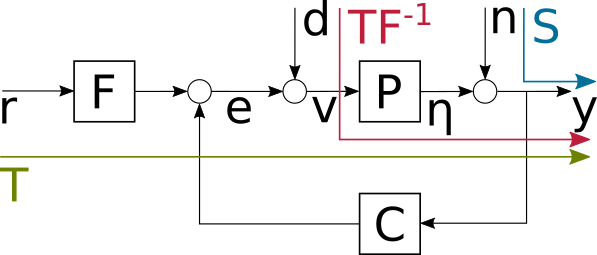
\includegraphics[width=0.9\textwidth]{./Graphics/2DOFCLOSEDLOOP.png}
\caption{Two Degree of Freedom Feedback Control}
\label{c:control:f:2dofclosedloop}
\end{minipage}
\end{figure}

In Fig. \ref{c:control:f:2dofclosedloop} further signals are added.The disturbances $\ve{d} \in \mathbb{R}^{n_y}$ are acting on the systems input, the signal $\ve{v} \in \mathbb{R}^{n_y}$ is the disturbed input of the plant. $\ve{y} \in \mathbb{R}^{n_y}$ is the plants output without measurement noise which will be referred to as real output. The measurement noise is given by $\ve{n} \in \mathbb{R}^{n_y}$. The superposition of noise and real output is $\ve{\eta}$ which will be referred to simply as output. The closed loop transfer function is given by:

\begin{align}
\begin{split}
\ve{y} &= \left[\ma{I} - \ma{G} \ma{K}_y\right]^{-1} \left[ \ma{G}\ma{K}_r \ve{y}_r + \ve{n} + \ma{G} \ve{d} \right]
\end{split}
\label{c:control:e:2dofclosedloop}
\end{align}
\nomenclature{$\ve{d}$}{Disturbance Vector of a Dynamical System}
\nomenclature{$\ve{n}$}{Measurement Noise Vector of a Dynamical System}

Eq. \ref{c:control:e:2dofclosedloop} relates the output of a system to the influences of set point, disturbances and measurement noise. 
Rewriting the equation as:

\begin{align}
\begin{split}
\ve{y} &= \ma{T}\ve{y}_r + \ma{S} \left[ \ve{n} + \ma{G} \ve{d} \right]
\end{split}
\label{c:control:e:sensitivityclosedloop}
\end{align}
defines the Sensitivity Function $\ma{S} = \left[ \ma{I} - \ma{G} \ma{K}_y\right]^{-1} \in \mathbb{C}^{n_y \times n_y}$ which relates the influences of measurement noise and load disturbance to the systems outputs. The Complementary Sensitivity Function $\ma{T} = \left[\ma{I} - \ma{G} \ma{K}_y\right]^{-1} \ma{G} \ma{K_r} \in \mathbb{C}^{n_y \times n_y}$ describes the response to the reference signal.Both Functions play an important role in the investigation of the systems Robustness and are connected to each other via $\ma{T} = \ma{S} \ma{G} \ma{K}_r$.\\

\section{Stability and Robustness of Feedback Control Systems}
\label{c:control:s:robustness}

The stability of dynamical systems is a key concept of control theory. In general, a system is said to be stable if all trajectories starting near a final state end in or near this state \cite[p.10]{Adamy2014}. Several measurements, e.g. Lyapunov based methods, exist to proof a system is stable, see \cite{Lunze2016},\cite{Lunze2014} or \cite{Adamy2014}. A necessary condition for a stable state $\ve{x}_S \in \mathbb{R}^{n_y}$ can be formulated for the system given in Eq. \ref{c:control:e:nonlinearsystem} as:

\begin{align}
\begin{split}
\ve{x}_S = \lbrace \ve{x} \in \mathbb{R}^{n_y} ~ | ~\ve{f}(\ve{x}) = \ve{0} \rbrace 
\end{split}
\label{c:control:e:StabilityCondition}
\end{align} 

Robustness refers in general to the stability of the system in presence of uncertainties and has been studied extensively, see e.g. \cite{Zhou1998},\cite{Zhou1996}, \cite{Doyle}.
To give a better understanding of the relevant points of the subject both SISO and MIMO cases are presented. \\

For any given SISO system with a transfer function $g : \mathbb{R} \mapsto \mathbb{C}$ we see from Eq. \ref{c:control:e:2dofclosedloop} that the behaviour of the output with respect to measurement noise and disturbances is strongly dependent on the sensitivity function. A necessary condition for the system to reach the reference is that disturbance and noise are attenuated  near the steady state. Furthermore the destabilizing effect due to uncertain signals can be quantified via the maximum of the sensitivity function. Therefore the Maximum Sensitivity is defined as:

\begin{align}
\begin{split}
M_S & = \max_\omega \left| S \right| \\
& \geq \left| \frac{1}{1 - g~k_y}\right|
\end{split}
\label{c:control:e:maxsensitivity}
\end{align}

With Eq. \ref{c:control:e:maxsensitivity} an upper boundary on the gain can be found and be used as a measure of robustness of the closed loop \cite[p.323 ff.]{Astrom2009}. The maximum sensitivity is also connected to the nyquist stability and the stability margin of a system via:

\begin{align}
\begin{split}
M_S &= \frac{1}{s_M} \\
&= \frac{1}{1 - \max_\omega \left| g ~k_y \right|}
\end{split}
\label{c:control:e:maxsensitivitynyquist}
\end{align}

Or rearranged to be:

\begin{align}
\begin{split}
\max_\omega \left| g~k_y\right| &= 1 - s_M
\end{split}
\end{align}

Due to Eq. \ref{c:control:e:maxsensitivitynyquist} the maximum gain of the open loop is limited by the maximum sensitivity. Hence, the critical point is only encircled iff the maximum sensitivity is zero. Hence the system is only stable in the sense of the Nyquist Criterion if the maximum sensitivity is sufficiently small.\\


\begin{figure}[h]\centering
\includesvg[width = \textwidth]{Maximum_Sensitivity.svg}
\caption{Illustration of the Connection between the maximum sensitivity, the open loop gain and the Nyquist Criterion}
\label{c:control:f:maxsensitivitynyquist}
\end{figure}


%\begin{figure}[H]
%  \centering
%  \def\svgwidth{\textwidth}
%  \import{MS.pdf_tex}
%%  \caption{Illustration of the maximum sensitivity of a given system}
%%  \label{c:identification:f:MaximumSensitivity}
%\end{figure}


While the maximum sensitivity is well defined for SISO systems, a MIMO system requires a more general approach due to the interconnection of the systems out- and inputs. A general condition is given by the Small Gain Theorem \cite[p.150 ff.]{Skogestad2005}. The theorem states, that a given feedback system is stable iff the open loop transfer function matrix is stable and its sufficient conditioned matrix norm is less than 1 over all frequencies.

\begin{align}
\lVert \ma{G} \ma{K}_y \rVert < 1 ~\forall \omega
\label{c:control:e:SmallGainTheorem}
\end{align}

Eq. \ref{c:control:e:SmallGainTheorem} can be used with several matrix norms and can be viewed as an MIMO Interpretation of the Nyquist Criterion. \\

For further robustness analysis, the concept of singular values has to be investigated. The singular value decomposition, see e.g. \cite[p.144 f.]{Zeidler2013},states that any matrix $\ma{G} \in \mathbb{C}^{n_a\times n_b}$ can be factorized such that

\begin{align}
\ma{G} &= \ma{U}\ma{\sigma}\ma{V}^*
\label{c:control:e:SVD}
\end{align}

Where $\ma{U} \in \mathbb{C}^{n_a \times n_a}$ and $\ma{V} \in \mathbb{C}^{n_b \times n_b} $ are unitary matrices representing the left and right eigenvectors of matrix. The matrix $\ma{\sigma} \in \mathbb{C}^{n_a \times n_b}$ is a rectangular, diagonal matrix consisting of the singular values $\sigma \in \mathbb{C}$ of $\ma{G}$. A practical point of view suggest a rotation of any given input vector via $\ma{V}^*$, distributing the magnitude of the input over the columns of $\ma{\sigma}$, where they are scaled according to the magnitude of the corresponding singular value. Then the scaled and rotated vector is once again rotated by $\ma{U}$ and distributed over the output vector. \\

\begin{figure}[H]
\begin{minipage}[b]{\textwidth}
\centering
\includesvg[width = \textwidth]{Bode_Singular_Value.svg}
\caption{Example for the maximum singular value as an upper limit to the gain}
\label{c:control:f:SVD}
\end{minipage}
\end{figure}



An example of this process is illustrated in Fig. \ref{c:control:f:SVD} for a system with two inputs $u_1,u_2$ and two outputs $y_1,y_2$. The output is bounded by the ellipsoid described by the maximum singular value $\overline{\sigma}$ and the minimum singular value $\underline{\sigma}$. The orientation and the magnitude of the outputs change depending on the frequency but will never exceed these limits. The singular values of a matrix are hence representing the highest possible gain for any given input if $\ma{U} = \ma{V}^* = \ma{I}$. With that, the induced 2-Norm for a matrix can be defined as:

\begin{align}
\begin{split}
\lVert \ma{G} \rVert_2 &= \frac{\lVert \ma{G}\ma{u}\rVert_2}{\lVert \ma{u} \rVert_2} \\
&= \max \sqrt{\lambda\left( \ma{G}^* \ma{G}\right)} \\
&= \overline{\sigma}
\end{split}
\label{c:control:e:MaxSingularValue}
\end{align}

\section{Gain Scheduling} % (fold)
\label{c:control:s:gainsched}

% section gain_scheduling (entrol:s:gainschednd)
%!TEX root = ../studentischeArbeiten.tex
\chapter{Process Models and System Identification}\label{c:identification}

The following chapter serves as an introduction to the modeling of energy and process plants with analogous models. Its secondary aim is to provide a short introduction to the field of system identification in general while giving an in-depth view of two simple but nonetheless very useful methods. 
\\

In Sec. \ref{c:identification:s:fotd} the first order time delay model is introduced. The parameters and key properties are introduced. Furthermore, an interpretation of the model error with respect to the dynamic behavior of the system is given. \\

Afterwards the first parameter estimation method is presented in Sec. \ref{c:identification:s:area}. The basic concept is explained and visualized. An algorithm in pseudo-code is provided to clarify the approach. \\

The second model based fitting process is explained in Sec. \ref{c:identification:s:relay}. Like earlier, important relations between the measured data are given to provide the necessary steps of estimating the parameters. \\

A critical review of both algorithms finishes the chapter in Sec.\ref{c:identification:s:review}. Drawbacks of both methodology are enlisted. It closes with recommending a procedure.\\

Since this chapter deals with system identification, a brief introduction to the subject is given in advance. To design a controller for a given process either a theoretical model based on physical laws or first principles, e.g. energy conservation, Newton's laws or the laws of thermodynamics, or an analogous model based on the measured relation between input and output is required. Since not all processes are well-fitted to be physically modeled, the field of system identification provides a vast toolbox for deriving the needed mathematical description. A good, practical approach towards the principles is given in \cite{Keesman2011}, while \cite{Isermann1992} and \cite{Isermann1992a} covers most of the techniques used today.An overview from a more philosophical and methodological perspective is \cite{Ljung2010}.\\

An important aspect of current techniques is the statistical evaluation of the signals measured. Many simplifications to these data processing procedures require the input to be statistical independent from itself and the output. While in theory possible, in reality a signal called pseudo random binary sequence (PRBS) is used.\\

The most important and common used algorithm is called Least squares (LS), e.g. \cite[p.62 ff.]{Keesman2011}. Here the estimation process is viewed as a regression problem. LS is a parameter based estimation approach, and able to estimate models up to nearly infinite order. Several enhancements have been provided so that the algorithm is both fast and effective while being able to handle even nonlinear models. Despite its many advantages, the need for a high order model is neither desirable nor effective. Dealing with PI/PID control requires a robust set of few parameter.\\

\section{First Order Time Delay Model}%
\label{c:identification:s:fotd}

As discussed earlier system identification enables the user to use various methods to process information to derive a suitable dynamical model.To ensure a deterministic, robust and simple controller, an identification based on a process model with simple dynamics is chosen. The reasons for this approach are based on the variety of the process itself as well as the algorithms used for determination of the controller parameters, see \cite{Astrom1995}, \cite{Astrom2006}.\\

The model structure used in the scope of the work is a given by the transfer function

\begin{align}
\begin{split}
\hat{G} &= \frac{\hat{K}}{\hat{T}s+1}e^{-\hat{L}s}
\end{split}
\label{c:identification:e:fotd_tf}
\end{align}

Eq. \ref{c:identification:e:fotd_tf} describes the function $\hat{G}: \mathbb{C} \mapsto \mathbb{C}$ in the s-plane and is called a first order time delay (FOTD) or first order plus deadtime (FOPDT) model, \cite[p.16]{Astrom1995}, \cite[p.20, p.26]{Astrom2006}, \cite{Fedele2009a}, \cite{Bi1999}.
The model gain $\hat{K} \in \mathbb{R}$ is the steady state gain of the system, a model time constant $\hat{T} \in \mathbb{R}^+$ and a model time delay $\hat{L} \in \mathbb{R}^+$ describe the dynamic gain and phase. Its representation as a differential equation is given to be

\begin{align}
\begin{split}
\hat{T}~\frac{dy}{dt} + y &= \hat{K} ~\sigma(t-\hat{L})~u
\end{split}
\label{c:identification:e:fotd_de}
\end{align}

The general solution for a step response acting on Eq.\ref{c:identification:e:fotd_de} is 

\begin{align}
\begin{split}
y &= \hat{K} ~\left( 1 - e^{-\frac{t- \hat{L}}{\hat{T}}}\right)~ \sigma(t-\hat{L}) ~u
\end{split}
\label{c:identification:e:fodt_dt}
\end{align}

The Heavyside step function $\sigma(t): \mathbb{R} \mapsto \mathbb{R}$ is defined as

\begin{align}
\begin{split}
\sigma(t) &= \begin{cases} 
      0 , ~t < 0 \\
      1, ~t \geq 0
   \end{cases}
\end{split}
\label{c:identificitaion:e:heavyside}
\end{align}

and hence models the delay acting on the connection between the output and the input. It is worth noting that in the special case of a SISO system a delay acting on the systems input or output is mathematical equivalent. However, for a given MIMO system model it can be of importance to model correctly where the delay intervenes. \\

An important characteristic with respect to the time behavior of the process is given by the normalized time $\tau, \left[0 \leq \tau \leq 1 \right] $ \cite[p.16]{Astrom1995}

\begin{align}
\begin{split}
\tau &= \frac{\hat{L}}{\hat{L}+\hat{T}}
\end{split}
\label{c:identification:e:normalizedtime}
\end{align}

Eq. \ref{c:identification:e:normalizedtime} gives the ratio of the delay and the sum of delay and time constant, called average residence time. It can be used as a rating regarding the difficulty of controlling the process, since a high normalized time indicates a delay dominance and hence a very difficult process to control. It can also be connected to the gain ratio \cite[p.27]{Astrom2006}.\\

Since the process model is of utmost interest for the overall process, a detailed investigation of its properties is conducted. This detailed description is started by investigating the model gain over the frequency. It is conventional to substitute the complex variable $s$ with the complex frequency $s~=~j~\omega$. The gain of the process model is hence given by:

\begin{align}
\begin{split}
\left| \hat{G} \right| &= \left| \frac{\hat{K}}{\hat{T}~j\omega+1} ~ e^{-\hat{L}~j\omega} \right| \\
&= \left| \frac{\hat{K}}{\hat{T}~j\omega+1} \right| \underbrace{\left| ~ e^{-\hat{L}~j\omega} \right|}_{\left|cos(\hat{L}\omega)+j~sin(\hat{L}\omega)\right| = 1} \\
&= \left| \frac{\hat{K}}{\hat{T}~j\omega+1} \right|
\end{split}
\label{c:identification:e:fotd_gain}
\end{align}

Eq.\ref{c:identification:e:fotd_gain} shows that the gain over the frequency of a FOTD model is equal to the gain of a first order system with the same time constant. The effect of the time delay is canceled due to the use of Euler's identity, which can be interpreted as an orthonormal rotation in the complex plane by an angle $\hat{L}\omega \in \mathbb{R}^+$ around the origin.\\

The systems phase can be described as

\begin{align}
\begin{split}
\hat{\varphi} &= \arg\left( \hat{G} \right) \\
&= \arg\left(\frac{\hat{K}}{\hat{T}~j\omega+1} ~ e^{-\hat{L}~j\omega} \right) \\
&= \arg\left(\frac{\hat{K}}{\hat{T}~j\omega+1}\right) + \arg\left( e^{-\hat{L}~j\omega}\right) \\
&= \arg\left(\frac{\hat{K}}{\hat{T}~j\omega+1}\right) - \hat{L}\omega
\end{split}
\label{c:identification:e:fotd_phase}
\end{align}

From Eq.\ref{c:identification:e:fotd_phase} the effect of the time delay follows directly. It imposes a negative shift in phase proportional to the frequency on the system. \\

Defining an error between the real, unknown system and the FOTD model requires the following identities of a general transfer function:

\begin{align}
\begin{split}
G &=  \frac{\sum_{i=0}^n a_i s^i}{\sum_{k=0}^m b_k s^k} \\
&= \frac{\prod_{i=0}^n \left( s^i - z_i \right)}{\prod_{k=0}^m \left( s^k-p_k\right)} 
\end{split}
\label{c:identification:e:general_tf}
\end{align}

Eq.\ref{c:identification:e:general_tf} shows the identities of a transfer function given as a polynomial in $s$ and its equivalent representation as a product of linear factor, see \cite[p.269 ff.]{Lunze2016}. The linear factorization consists of its zeros $z_i \in \mathbb{C}$ and poles $p_k \in \mathbb{C}$. Both identities will be useful due to the different properties of the gain and phase. Additionally it is assumed that the first order dynamics have been ideally identified. Hence, the error depends only on dynamics of higher order.\\

The relative error in Gain $\Delta_K \in \mathbb{C}$ can therefore be described as

\begin{align}
\begin{split}
\Delta_K &= \left| \frac{\hat{G}}{G}\right| \\
&= \underbrace{\left|\frac{\hat{K}}{\hat{T}~j\omega+1} \frac{\left(\ 1-p_0 \right)\left( s- p_1 \right)}{1-z_0} \right|}_{\approx 1} \left| \frac{\prod_{k=2}^m~(s^k-p_k)}{\prod_{i=1}^n~(s^i-z_i)} \right| \\
&\approx \left| \frac{\prod_{k=2}^m~(s^k-p_k)}{\prod_{i=1}^n~(s^i-z_i)} \right|
\end{split}
\label{c:identification:e:error_gain}
\end{align}

\begin{figure}[H]\centering
  \includesvg[width=\textwidth]{Graphics/Example_Bode_Gain}
  \caption{Gain of a high order transfer function and corresponding FOTD model}
  \label{c:identification:f:gain_fotd}
\end{figure}

From Eq.\ref{c:identification:e:error_gain} two important conclusions can be conducted. First, the error is small near the steady state iff the first order dynamics are estimated correctly. The steady state model is even error free, iff the true gain can be identified. Secondly, the error will increase dramatically for higher order dynamics since the model is not able to project these frequencies in an adequate manner. Another source of error can be found in low order zeros of the system, which will result in an infinite error of the gain. The gain error is visualized in Fig.\ref{c:identification:f:nyquist_fotd}. Here a high order system with a dominant first order dynamics is approximated by a FOTD process model. The gain is nearly identical until the point $\lbrace[2,-j6\rbrace]$. Here the system models time delay rotate the real and imaginary part and hence transforms the position of the trajectory. \\

\begin{figure}[H]\centering
  \includesvg[width = \textwidth]{Graphics/Example_Nyquist_Plot}
  \caption{Nyquist diagram of high order transfer function and corresponding FOTD model}
  \label{c:identification:f:nyquist_fotd}
\end{figure}

Likewise, the relative error in phase $\Delta_\varphi \in \mathbb{C}$ is given as:

\begin{align}
\begin{split}
\Delta_\varphi &= \arg\left(\frac{\hat{G}}{G}\right) \\
&= \arg\left(\underbrace{\frac{\hat{K}}{\hat{T}~j\omega+1} \frac{\left(\ 1-p_0 \right)\left( s- p_1 \right)}{1-z_0}}_{\approx 1} \frac{\prod_{k=2}^m~(s^k-p_k)}{\prod_{i=1}^n~(s^i-z_i)}e^{-\hat{L}~s} \right)\\
&= -L~\omega + \arg\left(\frac{\prod_{k=2}^m~(s^k-p_k)}{\prod_{i=1}^n~(s^i-z_i)}\right)
\end{split}
\label{c:identification:e:error_phase}
\end{align}

Eq. \ref{c:identification:e:error_phase} gives an important insight to the function of the time delay. It compensates for the higher order dynamics in phase, effectively reducing the error in phase. An example is given in Fig.\ref{c:identification:f:phase_fotd}. In Fig. \ref{c:identification:e:error_phase} shows the ability of the approximation to mimic the phase of the real process. Until $\omega \approx 0.13 \frac{rad}{s}$ the phase of the system model is nearly equivalent to the original system. After crossing this frequency, the model approximates a phase less than that of the original system, which is identical with a conservative estimate of the dynamic behavior.


\begin{figure}[H]\centering
  \includesvg[width=\textwidth]{Graphics/Example_Bode_Phase}
  \caption{Phase of High Order Transfer Function and Corresponding FOTD model}
  \label{c:identification:f:phase_fotd}
\end{figure}


\section{Integral Fitting Approach}
\label{c:identification:s:area}

The first algorithm to estimate the parameter of the model is based on inherent knowledge of the time behavior of the model. These properties described in the section can be found in e.g. in \cite{Bi1999}, \cite{Fedele2009a} and are part of mostly any undergraduate course in control theory. The experiment providing the needed data is a step response around the working point. The algorithm depends on the collected data of the input, the output and the time. It processes the data by evaluating several numerical integrals and connects the outcomes to the process parameters.\\

At first, the difference between the settling value of the output, $y(\infty)$, and the current value, $y(t)$, is computed over time

\begin{align}
\begin{split}
\int_0^\infty \left[ y(\infty)-y(t) \right] ~dt &= \int_0^\infty \left[ y\left(\infty \right) - \hat{K} ~\left( 1 - e^{ -\frac{t- \hat{L}}{\hat{T}} } \right)~ \sigma(t-\hat{L}) \right] ~dt \\
&= \hat{K} \int_0^{\hat{L}} \sigma(t) ~dt + \hat{K} ~\int^{\infty}_0 e^{ -\frac{t}{ \hat{T} } } ~dt \\
&= \hat{K}~\hat{L} + \hat{K} \left( -\hat{T} e^{-\frac{t}{\hat{T}}}\right) \Bigg\rvert^\infty_0 \\
&= \hat{K}~\left(\hat{T}+\hat{L}\right) \\
&= \hat{K}~\hat{T}_{ar}
\end{split}
\label{c:identification:e:area_tar}
\end{align}

In Eq.\ref{c:identification:e:area_tar} the average residence time $\hat{T}_{ar} \in \mathbb{R}^+$ is calculated from the integral. To simplify the equation above the linearity of the integral has been employed. Additionally the properties of the Heavyside function enabled a change in the lower boundary, hence the simplification.\\

Further exploitation of Eq. \ref{c:identification:e:fodt_dt} leads to the following integral

\begin{align}
\begin{split}
\int_0^{\hat{T}_{ar}} y(t) ~dt &= \int_0^{\hat{T}_{ar}} \left[ \hat{K} ~\left( 1 - e^{-\frac{t- \hat{L}}{\hat{T}}}\right)~ \sigma(t-\hat{L}) \right] ~dt \\
&= \int_{\hat{L}}^{\hat{T}_{ar}} \left[ \hat{K} ~\left( 1 - e^{-\frac{t}{\hat{T}}}\right) \right]~dt \\
&= \hat{K} \left( t + \hat{T} e^{-\frac{t}{\hat{T}}} \right) \Bigg\rvert_{\hat{L}}^{\hat{T}_{ar}} \\
&= \frac{\hat{K}}{e} \hat{T}
\end{split}
\label{c:identification:e:area_t}
\end{align}

At last, the gain $\hat{K}$ has to be computed. With the common definition, e.g. given in \cite[p.213]{Lunze2016}, the parameter can be computed using

\begin{align}
\begin{split}
\hat{K} &= \lim_{t\mapsto \infty} \frac{y(t)-y(0)}{u(t)-u(0)}
\end{split}
\label{c:identification:e:area_gain}
\end{align}

This interpretation is rooting in the final value theorem. Using Eq. \ref{c:identification:e:area_gain} in combination with the other two relations one is able to compute all needed parameters.\\

Assuming a disturbed output $\eta$ as described earlier, where measurement noise is added to the real output, one can see the benefits of using Eq.\ref{c:identification:e:area_tar} and \ref{c:identification:e:area_t}. Since the expected value / mean of the noise is given by 

\begin{align}
\begin{split}
\int_{-\infty}^{\infty} \eta \left( t \right) dt&= \int_{-\infty}^{\infty} \left[ y \left(t \right) + n\left(t\right) \right] dt \\
&= \int_{0}^{\infty}  y \left(t \right) dt + \underbrace{\int_{0}^{\infty} n\left(t\right) dt }_{= 0}\\
&= \int_{0}^{\infty}  y \left(t \right) dt
\end{split}
\label{c:identification:e:integral_noisechancel}
\end{align}

From Eq. \ref{c:identification:e:integral_noisechancel} follows that measurement noise has no effect on the average residence time and the time constant. Hence, both model parameter can robustly be estimated. In contrast, Eq.\ref{c:identification:e:area_gain} is strongly reliant on the signal to noise ratio. If the system is strictly monotone, meaning its outputs is only increasing over time, one can use an average over a measured time interval $\Delta T \in \mathbb{R}^+$. The model gain can be estimated with

\begin{align}
\begin{split}
\hat{K} &= \lim_{\Delta T\mapsto \infty} \frac{1}{\Delta T} \frac{\int_{0}^{\Delta T} \left[ y \left( t\right) - y\left(0\right)\right] dt}{u \left( t \right)-u \left( 0 \right)}
\end{split}
\label{c:identification:e:area_averagegain}
\end{align}

The system of equations as described above are called area-based methods, \cite{Fedele2009a}, with regards to its visualization displayed in Fig.\ref{c:identification:f:Area}, where the response to a unit step of a FOTD system is shown. Another, likewise valid understanding is given as the minimization of the integral of the error between the real system and the model over time.\\

\begin{figure}[H]\centering
\includesvg[width = \textwidth]{Graphics/FOTD_Area}
\caption{Interpretation of the Integral Fitting Approach using Areas given by a unit step response}
\label{c:identification:f:Area}
\end{figure}

However, the algorithm described above is not robust. It only converges iff the systems gain is equivalent with the infinity norm of the output. This resembles a dominant steady state gain. In other words, the integral Eq. \ref{c:identification:e:area_tar} must be positive definite, meaning the time response of the process is monotonic increasing. To ensure this, several options are available. \\

Since a conservative estimation of the system will result in a robust controller, the gain is preferred to be calculated to big. Likewise a smaller phase increases the immunity to disturbance. Hence, a conservative bound is established with truncating the data so that the maximum output is corresponding to the end of measurement. The systems gain will be computed as

\begin{align}
\begin{split}
\hat{K} &= \lim_{t\mapsto t^*} \frac{y(t^*)-y(0)}{u(\infty)-u(0)}, ~ y(t^*) = \sup_{0 \leq t \leq \infty} y(t)
\end{split}
\label{c:identification:e:area_sup_gain}
\end{align}

Eq. \ref{c:identification:e:area_sup_gain} defines the gain as the ratio between the supremum of the measurement data and the change in input. This results in a positive semidefinite value of the integral given by Eq.\ref{c:identification:e:area_tar}. Furthermore, the results in two extreme cases. The algorithm can provide the real system, iff the output data is monotonically increasing. With that, the supremum of the collected data is equal to the final value and Eq.\ref{c:identification:e:area_sup_gain} converges to Eq. \ref{c:identification:e:area_gain}. On the other hand the system is identified as a (scaled) step response or a strictly proportional element, iff the supremum is equal to the first collected data point. An illustration of the former reasoning is given in Fig.\ref{c:identification:f:SupGain}, where some responses of a not monotonic behavior are identified using the supremum gain.\\

\begin{figure}[H]\centering
\includesvg[width = \textwidth]{Graphics/Area_Fitting}
\caption{Identification of the Systems Gain using the Supremum of the Step Response}
\label{c:identification:f:SupGain}
\end{figure}

\section{Asymmetric Relay Experiment}
\label{c:identification:s:relay}

Another class of experimental methods based on a priori model structure is called relay experiments. These methods have been introduced in the early 1980's, ZITIEREN, and have since then been investigated, developed and used in an industrial context, see . The following section is mainly based on the recent works \cite{Berner2016a}, \cite{Berner2015} and \cite{Berner2014a}.\\

The key concept to estimate the needed parameters is based on the systems response to an (asymmetric) relay input, forcing a semi-stationary limit cycle. This behavior is illustrated in FIG. .\\

HIER FIGURE \\

The block diagram used to generate the output is shown in FIG. \\

HIER FIGURE \\

The relay generating the input signal of the process can be described as follows:

\begin{align}
\begin{split}
u(t) = \begin{cases}
u_H &~e(t) > h, ~\dot{e}(t) > 0 \\
u_H &~e(t) < h, ~\dot{e}(t) < 0\\
u_L &~e(t) > -h,~\dot{e}(t) > 0\\
u_L &~e(t) < -h, ~\dot{e}(t) < 0
\end{cases}
\end{split}
\label{c:identification:e:relay_output}
\end{align}

In Eq. \ref{c:identification:e:relay_output} the output switches between an upper and lower limit, $u_H, u_L \in \mathbb{R}, u_H \geq u_L$ depending on the hysteresis $h \in \mathbb{R}^+$, the error of the signal and its time derivative. Iff the relation $\left| u_H \right| = \left| u_L \right|$ holds true, the relay is called symmetric, if not it is an asymmetric relay, with $\left| u_H \right| > \left| u_L \right|$. Note that the system of equations above can be formulated with respect to the former value of itself. Since the process is defined around a set point $y_R \in \mathbb{R}$ it is useful to define the corresponding input $u_R \in \mathbb{R} | y = y_R$. Hence, the difference in input is given by $\delta u_H = \left| u_H-u_R \right|$ and $\delta u_L = \left| u_L - u_R \right|$.\\

From FIG a difference the period $t_P = t_{on} + t_{off}\in \mathbb{R}^+$ consisting of the sum of the half-periods $t_{on} \in \mathbb{R}^+ | u = u_H$ and $t_{off} \in \mathbb{R}^+ | u = u_L$.\\

To estimate the parameter set of a FOTD model, the normalized time delay is approximated according to \cite[p.26 f.]{Berner2015}:

\begin{align}
\begin{split}
\tau &= \frac{\hat{L}}{\hat{T}+\hat{L}} \\
 &= \frac{\gamma - \rho}{ \left(\gamma - 1\right)\left(0.35~\rho+0.65\right)}
\end{split}
\label{c:identification:e:relay_normalizedtime}
\end{align}

With the half-period ratio $\rho = \frac{\max\left(t_{on},t_{off} \right)}{\min\left(t_{on},t_{off} \right)} ~\in \mathbb{R}^+$ and $\gamma = \frac{\max\left(\delta u_H, \delta u_L \right)}{\max\left(\delta u_H, \delta u_L \right)}$ being the asymmetry level of the relay. Notice the impact of an symmetry in the relay, since it immediately follows that Eq. \ref{c:identification:e:relay_normalizedtime} is singular if the amplitudes are symmetric. Furthermore, the delay is zero estimated to zero iff the half-period ratio is equal to the asymmetry level.\\

To compute the gain the following relationship can be utilized:

\begin{align}
\begin{split}
\hat{K} &= \frac{\int_{t_P} y(t)-y_R~dt}{\int_{t_P} u(t)-u_R~dt} \\
&= \frac{\int_{t_P} y(t)-y_R~dt}{ \left( u_H -u_R \right)~t_{on} - \left( u_L - u_R \right)~t_{off}} 
\end{split}
\label{c:identification:e:relay_gain}
\end{align}

Eq. \ref{c:identification:e:relay_gain} calculates the gain as a ratio between the quasi stationary limit cycles. The importance of the asymmetry is again visible by investigating the denominator. Singularities of Eq. \ref{c:identification:e:relay_gain} are given iff the quantities of turn-on and turn-off phase are either equal, which resembles a symmetric relay, or in a suitable ratio to each other.\\

The time constant of the model can be calculated using one of the following equations:

\begin{align}
\begin{split}
t_{on} &= \hat{T}~ \log\left( \frac{h/\hat{K}-\delta u_L + e^\frac{\hat{L}}{\hat{T}} \left(\delta u_H + \delta u_L \right) }{\delta u_H - h/\hat{K}}\right) \\
t_{off} &= \hat{T}~  \log\left( \frac{h/\hat{K}-\delta u_H + e^\frac{\hat{L}}{\hat{T}} \left(\delta u_H + \delta u_L \right) }{\delta u_L - h/\hat{K}}\right) 
\end{split}
\label{c:identification:e:relay_time}
\end{align}

Eq. \ref{c:identification:e:relay_time} can be exploited by using the Eq. \ref{c:identification:e:relay_normalizedtime} by solving it for the ratio between time delay and time constant. Hence, the system can be used to computed $\hat{T}$ and thus $\hat{L}$. \\

While computing the gain is robust to measurement noise, see Eq. \ref{c:identification:e:integral_noisechancel}, an immediate disadvantage can be seen from the computation of the systems delay and time constant. If the delay of a real process is small, the experiment does give parameter in adequate error limit \cite{Berner2016a} and different process models need to be used, eventually requiring numerical parameter fitting \cite[p. 31 ff.]{Berner2015}. Furthermore the needed experimental parameter, such as asymmetry and hysteresis, take influence on the result of the estimation \cite{Berner2016a} and have to be chosen according to the process itself. Hence, several experiments are needed to fully identify the systems parameter. At last, the 

\section{Review}
\label{c:identification:s:review}

Above two important and well known fitting techniques based on structural knowledge of a FOTD and hence mathematical formulations of the model have been introduced. Even though both methods are used throughout industry, there are certain drawbacks to each method which should be considered.\\

While the asymmetric relay process introduced in Sec. \ref{c:identification:s:relay} is especially useful in determining the model parameter with a quasi stationary limit cycle it requires several in depth adjustments and process knowledge. Adjusting the asymmetry and the hysteresis in a proper way has an notable impact on the result \cite{Berner2016a}. The noise level, process gain and sampling times influences the algorithm. Hence, prior experiments have to be made. Additionally, not every process is suited to be estimated in the described way \cite{Berner2016a},\cite{Berner2015}. Depending on the normalized time delay several changes in model structure or additional experiments must be performed. Depending on the process time scale and the requirement of a quasi stationary cycle the experiment can require several hours.\\

Apparently, the parameter estimation based on area methods as given in Sec.\ref{c:identification:s:area} has the disadvantage of both requiring a steady process output. Hence, the parameter can not fully be estimated. Another drawback is given by the assumption of a dominant static gain. The error in gain and phase get higher by using Eq.\ref{c:identification:e:area_sup_gain}.\\

However, both methods are - up to a certain degree - independent from measurement noise and well established. Due to the simplicity and robustness of the area based identification it is commendable to use this algorithm. 

%!TEX root = ../studentischeArbeiten.tex
\chapter{Multivariable PI/PID Controller Design}%
\label{c:controller}

Chapter \ref{c:controller} gives an overview about basic concepts used in the context of this work. The fundamentals can be found in the literature already mentioned in Ch.\ref{c:control}. Additional information on process control and especially PID control is given in \cite{Astrom1995} and \cite{Astrom2006}. The concepts of decoupling control are explained in great detail in \cite{Wang2006}.\\

The chapter starts in Sec. \ref{c:controller:s:AMIGO} with a brief explanation of the tuning rules used to derive the parameter set of the controller. \\

Afterwards a method to evaluate the input output coupling in multivariable process models is explained in Sec.\ref{c:controller:s:rga}. Some interesting properties are explained in detail.\\

In Sec.\ref{c:controller:s:decoupling} the key concept of this work is explained. Starting by introducing a method presented in \cite{Astrom2001a} and developing it to an equivalent, but more useful representation, the design of decoupled control loops is given. \\

\section{AMIGO Tuning Rules} % (fold)
\label{c:controller:s:AMIGO}

Many rules to design proportional-integral-derivative controller exist \cite[p.158 ff.]{Astrom2006}. The most famous set of rules has been developed by Ziegler and Nichols. Other rules, such as Cohen-Coon, can be named as well. The simple set of rules, derived by experimental procedures, have since then been reused for several tuning approaches \cite[p.169]{Astrom2006}. Other, analytical methods e.g. Pole Placement or Haalman's Method exists as well, but require a detailed model of the process.  In \cite[p.206 ff.]{Astrom2006} a robust loop shaping based on optimization has been introduced. A key concept is illustrated by the robustness region of a given process, depending on the controllers parameter set and the constrain in form of a maximum sensitivity. These optimization process lead to the M constrained Integral Gain Optimization (MIGO) method \cite[p.217]{Astrom2006}, an iterative algorithm calculating the needed parameter values.
The Approximate MIGO (AMIGO) tuning rules have been introduced in \cite[p.225 ff.]{Astrom2006}. They are derived by applying the MIGO algorithm to a test batch while demanding $M_S = 1.4$ . All processes of the test batch are approximated by a sufficiently analogous model, namely a integrating process with delay, a FOTD model , as described in Sec.\ref{c:identification:s:fotd} and a second order model. \\

The investigation of the optimization results can be condensed into the following set of equations for a simple proportional-integral controller based on a FOTD model approximation:

\begin{align}
\begin{split}
K_P &= \frac{0.15}{\hat{K}}+ \left(0.35 - \frac{\hat{L}~\hat{T}}{\left( \hat{L}+\hat{T} \right)^2} \right) \frac{\hat{T}}{\hat{K}~\hat{L}} \\
T_I &= 0.35~ \hat{L} + \frac{13~\hat{L}~\hat{T}^2}{\hat{T}^2 + 12~\hat{L}~\hat{T}+7 \hat{L}^2}
\end{split}
\label{c:controller:e:amigo_pi}
\end{align}

Eq.\ref{c:controller:e:amigo_pi} defines the proportional gain of the controller $K_P \in \mathbb{R}$ and the integral time $T_I \in \mathbb{R}$.\\

Additionally, the optimal calculated parameter of a proportional-integral-derivative controller are formulated as

\begin{align}
\begin{split}
K_P &= \frac{1}{\hat{K}} \left( 0.2 + 0.45~ \frac{\hat{T}}{\hat{L}}\right)\\
T_I &= \frac{0.4~\hat{L}+0.8~\hat{T}}{\hat{L}+0.1~\hat{T}}\hat{L}\\
T_D &= \frac{0.5~\hat{L}~\hat{T}}{0.3~\hat{L}+\hat{T}}
\end{split}
\label{c:controller:e:amigo_pid}
\end{align}

Eq.\ref{c:controller:e:amigo_pid} introducing the derivative Time $T_D \in \mathbb{R}$.\\

The AMIGO rules presented above hold several properties described in \cite[p.229 ff.]{Astrom2006}. Important advice in the context of this work is given in form of a recommendation for set-point weighting \cite[p.229 f., p.235 ff.]{Astrom2006} and a drawback with respect to lag dominance \cite[p.231 ff.]{Astrom2006}.\\ 

In \cite[p.253 ff.]{Astrom2006} the detuning process is described. Since detuning is an essential element of the overall design procedure, as shown later, the method will be explained here. It is used if the controller is acting to fast and hence producing unwanted overshoot. To reduce this effect, the controller parameter need to be scaled to smaller values while ensuring the stability. Therefore an algorithm describing the adjustment of the gains with respect to each other is needed.\\

Based on the maximum sensitivity the following dimensionless factors are defined 

\begin{align}
\begin{split}
\alpha_D &= \frac{M_S-1}{M_S}\\
\beta_D &= M_S \frac{M_S+\sqrt{M_S^2 -1}}{2} 
\end{split}
\label{c:controller:e:amigo_factor}
\end{align}

Eq. \ref{c:controller:e:amigo_factor} defines the factors needed for calculating the new value of the integral gain $K_I = \frac{K_P}{T_I}$ according to

\begin{align}
\begin{split}
K_I^{i+1} &= \begin{cases}
	K_I^i \frac{\alpha_D + K_P^{i+1} \hat{K}}{\alpha_D + K_P^{i} \hat{K}} ~, K_P^{i+1} \hat{K} \geq \frac{K_I^{i}\hat{K}\left(\hat{L}+\hat{T}\right)}{\beta_D \left( \alpha_D + K_P^{i+1} \hat{K}\right)} - \alpha_D\\
	\beta_D \frac{\left( \alpha_D + K_P^{i+1} \hat{K} \right)^2}{\hat{K} \left( \hat{L}+ \hat{T} \right)}~, K_P^{i+1} \hat{K} < \frac{K_I^{i}\hat{K}\left(\hat{L}+\hat{T}\right)}{\beta_D \left( \alpha_D + K_P^{i+1} \hat{K}\right)} - \alpha_D\\
\end{cases}
\end{split}
\label{c:controller:e:amigo_detune}
\end{align} 

Eq.\ref{c:controller:e:amigo_detune} is derived by investigating the robustness of a FOTD sysem in dependence of the parameter of the controller and approximation of the same.\\

\section{Interaction Measures of Multivariable Processes} % (fold)
\label{c:controller:s:rga}

Current controller design in the problem set of this work is mostly relying on the assumption that the system is behaving like an assembly of single input single output processes. It is based not on holistic approaches but on calculating the parameter solely with regards to the current loop. To choose the right pairing of in- and outputs resembling with a maximal dominance over the output the relative gain array (RGA) has been introduced by \cite{Bristol1966}. Other measurements and indicators, like the Hankel Singular Values, Hankel Interaction Indexes or the Participation Matrix, have been developed as well, see e.g. QUELLEN. The RGA however is used intensively in industry and described in literature \cite[p. 88 ff.]{Skogestad2005}, \cite[p.219 ff.]{Glad2000}. The RGA is defined as

\begin{align}
\begin{split}
\Lambda\left(\ma{G}\right) &= \ma{G} \circ \ma{G}^{-T}
\end{split}
\label{c:controller:e:rga}
\end{align}

The RGA $\Lambda:\mathbb{C}^{n_y \times n_y},\mathbb{C}^{n_y \times n_y} \mapsto \mathbb{C}^{n_y \times n_y}$ as defined in Eq.\ref{c:controller:e:rga} is given by the hadamard product of the transfer function matrix and its transposed inverse. It can be interpreted as a ratio between open loop control and closed loop control \cite[p.221]{Glad2000}. Most commonly, the RGA is computed in the steady state of the system, but the elements near the crossover frequency give likewise useful information. To illustrate this, consider a simple system with a steady state gain and its inverse given by

\begin{align}
\begin{split}
\left|\ma{G}|_{s=0}\right| &= \begin{bmatrix}
2 & -1 \\
5 & 10
\end{bmatrix} \\
\left| \ma{G}|_{s=0}^{-1} \right| &= \frac{1}{25} \begin{bmatrix}
10 & 1 \\
-5 & 2
\end{bmatrix}
\end{split}
\end{align}

The corresponding RGA is given by:

\begin{align}
\begin{split}
\Lambda(\ma{G}) &= \begin{bmatrix}
2 & -1 \\
5 & 10
\end{bmatrix} ~\frac{1}{25} \begin{bmatrix}
10 & 1 \\
-5 & 2
\end{bmatrix}^T \\
&= \frac{1}{25}~\begin{bmatrix}
2 & -1 \\
5 & 10
\end{bmatrix} ~ \begin{bmatrix}
10 & -5 \\
1 & 2
\end{bmatrix} \\
&= \frac{1}{25} \begin{bmatrix}
20 & 5 \\
5 & 20
\end{bmatrix}\\
&= \begin{bmatrix}
0.8 & 0.2 \\
0.2 & 0.8
\end{bmatrix}
\end{split}
\end{align}

Which indicates a pairing of the main diagonals, since the matrix is diagonal dominant. In other terms, the system in closed loop control will behave nearly like the open loop control system. To discuss the RGA at crossover frequency, assume the system is in reality described by:

\begin{align}
\ma{G}(s) = \begin{bmatrix}
\frac{2}{s +1} & \frac{5s-1}{s +1} \\
\frac{5}{s +1} & \frac{10}{s +1}
\end{bmatrix}
\end{align}

The gain crossover frequency of MIMO systems is defined as the first frequency at which any of the transfer functions crosses the unit gain, or equivalently zero dB, from above \cite[p.37]{Skogestad2005}. Assuming normalized gains $k_{ij}= 1$ holds that $\omega_C = \min(\frac{1}{T_{ij}})$for any pure lag systems. Hence, the estimated crossover frequency of above system is $\omega_C \approx 1$. The systems gain and its inverse is given by the complex matrices:

\begin{align}
\begin{split}
\left|\ma{G}|_{s=j}\right| &= \frac{1}{j+1} \begin{bmatrix}
2 & 5j-1 \\
5 & 10
\end{bmatrix} \\
\left| \ma{G}|_{s=j}^{-1} \right| &\approx \begin{bmatrix}
0.000 & 0.200 \\
0.000 & 0.000
\end{bmatrix} + j~\begin{bmatrix}
0.400 & 0.040 \\
0.200 & 0.080 
\end{bmatrix}
\end{split}
\end{align}

The complex valued RGA of the system at the given frequency computes to be:\\

\begin{align}
\Lambda(\ma{G}|_{s=j}) = \begin{bmatrix}
0.400 & 0.600 \\
0.600 & 0.400 
\end{bmatrix}
+ j~\begin{bmatrix}
0.400 & -0.400 \\
-0.400 & 0.400
\end{bmatrix}
\end{align}

Which indicates a cross pairing over the minor diagonal of the system, since the real parts of the matrix are dominant.\\

Interesting properties of the RGA can be found in literature, eg. \cite{Skogestad2005}, \cite{Astrom1995}, \cite{Astrom2006}. However, the connection between the condition number $\kappa_C:~\mathbb{R},\mathbb{R} \mapsto \mathbb{R}$ and the RGA explained in \cite[p.88 f.]{Skogestad2005} is worth noticing. The condition number is given as

\begin{align}
\begin{split}
\kappa_C &= \frac{\overline{\sigma}(\ma{G})}{\underline{\sigma}(\ma{G})} \\
&= \overline{\sigma}(\ma{G}) \overline{\sigma}(\ma{G}^{-1})
\end{split}
\label{c:controller:e:condtion_number}
\end{align}

with the $\underline{\sigma} = \min(\sigma)$ being the lower bound of the singular values of a transfer function matrix. Eq.\ref{c:controller:e:condtion_number} can be interpreted as an index for the balance, meaning the ratio of the biggest and smallest possible gain, of a process. Furthermore, it can be interpreted as a measure of equivalence between the input-output relationship represented by the transfer function matrix. Hence, very large or very small condition numbers are not desirable and indicate a very poor performance. It can be minimized using scaling matrices best to be chosen by physical meaningful interpretations \cite[p.87]{Skogestad2005}. The sum norm of the RGA, meaning the sum over all elements of $\Lambda(\ma{G})$, is close to this minimal realizable value. Hence, large elements of the RGA indicate an ill-conditioned process.\\ 

Investigating the RGA leads to several conclusions about the optimal pairing of inputs and outputs. A selection with respect to this work is presented in the following.\\

If the elements of the RGA are large around the crossover frequency, a decoupler or inverse based controller should not be used \cite[p. 89]{Skogestad2005}, where large is corresponding to values $\geq 10$. Here the robustness to the uncertainty of inputs is not given \cite[p.243]{Skogestad2005}. If an element of the RGA calculated around steady state is negative, the decentralized controller tend towards instability \cite[p.90, p.447]{Skogestad2005}. \pagebreak

\section{Decoupling of Multivariable Processes} % (fold)
\label{c:controller:s:decoupling}

Designing controller for multivariable processes has inevitable challenges. Since a general MIMO plant consists of a main coupling, represented in the main diagonal of the transfer function matrix, and cross coupling given by the minor elements of the transfer function function matrix. An illustration of this problem is given in FIG. where both forward and backward coupling is pictured in a block diagram.\\

\begin{figure}[h]
\begin{minipage}[t]{0.45\textwidth}
\includesvg[width = \textwidth]{Graphics/Coupling_Forward}
\caption{Coupling in P-canonic structure}
\label{c:controller:f:pcanon}
\end{minipage}%
\hspace{0.05\textwidth}
\begin{minipage}[t]{0.45\textwidth}
\includesvg[width = \textwidth]{Graphics/Coupling_Backward}
\caption{Coupling in V-canonic structure}
\label{c:controller:f:vcanon}
\end{minipage}
\end{figure}


By closing a feedback loop a connection between these two elements is made out of necessity. Hence, the overall performance and robustness of a closed loop is influenced by the cross couplings between the inputs and outputs. To achieve better results regarding these two major aspects of the control paradigm, several techniques can be used solely or in combination to reduce the influence of the minor diagonal entries.\\


\subsection{Decoupling Control proposed by Astr\"om et.al.}
\label{c:controller:sub:astrom}

A method for the design of decoupling controllers is proposed in \cite{Astrom2001a} and \cite{Astrom2006}. A diagonal controller $\ma{K}^*$ which limits the interaction near the steady state of the plant within certain limitations is designed. To achieve this behavior a decoupler $\ma{D} \in  \mathbb{R}^{n_y \times n_y}$ is introduced. A static decoupling is proposed such that $\ma{D} = \ma{G}^{-1}|_{s=0}$ that transforms the system with the mapping $\ma{G} \ma{D} = \ma{G}^* \in \mathbb{R}^{n_y \times n_y}$. Since the decoupler is defined to be the inverse of the steady state gain, the steady state of the transformed system is given by the identity matrix $\ma{I} \in \mathbb{R}^{n_y \times n_y}$. The block diagram of the decoupled system is given in Fig.\ref{c:controller:f:decoupledsystem}.

\begin{figure}[h!]
\centering
\includesvg[width = .8\textwidth]{Graphics/Decoupled_System}
\caption{Block diagram of the decoupled system}
\label{c:controller:f:decoupledsystem}
\end{figure}

The resulting closed loop of the transformed system with a setpoint controller $\ma{K}_r$ and a feedback controller $\ma{K}_y$ is given by: 

\begin{align}
\begin{split}
\ma{H} &=  \left[ \ma{I}  - \ma{G} \ma{K}_y \right]^{-1} \ma{G} \ma{K}_r \\
&= \left[ \ma{I}  - \ma{G} \ma{D} \ma{K}_y^* \right]^{-1} \ma{G} \ma{D} \ma{K}_r^* \\
	 &= \left[ \ma{I}  - \ma{G}^* \ma{K}_y^* \right]^{-1} \ma{G}^* \ma{K}_r^*
\end{split}
\label{c:controller:e:closedloopastrom}
\end{align}
\nomenclature{$\ma{H}$}{Closed Loop Transfer Function}

Eq. \ref{c:controller:e:closedloopastrom} gives various important transformations between the controller and system of the original identified system and the new transformed system.The diagonal controller $\ma{K}^*$, designed based on the decoupled system $\ma{G}^*$ is connected to the controller of the original system via $\ma{K}^* = \ma{D} \ma{K}$.\\ 

A Taylor series around the steady state of the  transformed system is given by:

\begin{align}
\begin{split}
\ma{G}^* &= \sum_{i=0}^\infty \frac{d^i}{ds^i} \ma{G}^* |_{s=0} \frac{s}{i!} \\
&= \ma{I} + s \ma{\Gamma}^* + \ma{\mathcal{O}}\left(s^2\right) \\
&\approx \ma{I} +  \ma{\Gamma}^* s \\
&\approx \ma{I} + \left( \ma{\Gamma}^*_D + \ma{\Gamma}^*_A \right) s
\end{split}
\label{c:controller:e:taylor}
\end{align}

In Eq.\ref{c:controller:e:taylor} the coupling for small frequencies can be described via the coupling matrix $\ma{\Gamma}^* = \left( \gamma_{ij}^* \right)\in \mathbb{R}^{n_y \times n_y}$. The matrix consists both of diagonal and anti diagonal entries $\ma{\Gamma}^* = \ma{\Gamma}^*_D + \ma{\Gamma}^*_A$ which describes the small signal behavior of the system, represented by the first order of the series sufficiently.\\

Substitute Eq.\ref{c:controller:e:taylor} in the numerator of Eq. \ref{c:controller:e:closedloopastrom} holds:

\begin{align}
\begin{split}
\ma{H} &\approx \left[ \ma{I}  - \ma{G}^* \ma{K}_y^* \right]^{-1} \left[ \ma{I} +  \ma{\Gamma}^* s \right] \ma{K}_r^* \\
  &\approx \left[ \ma{I}  - \ma{G}^* \ma{K}_y^* \right]^{-1} \left[ \ma{I} + \left( \ma{\Gamma}^*_D + \ma{\Gamma}^*_A \right) s\right] \ma{K}_r^* \\
\end{split}
\end{align}

The anti diagonal entries are given by

\begin{align}
\begin{split}
\ma{H}_A &\approx \left[ \ma{I}  - \ma{G}^* \ma{K}_y^* \right]^{-1} \left[\ma{\Gamma}_A^* s \right] \ma{K}_r^*
\end{split}
\end{align}

According to \cite{Astrom2001a}, every entry of the matrix $\ma{H}_A = (h_{ij})~\forall i \neq j \in \mathbb{R}^{n_y \times n_y} $ simplifies to:

\begin{align}
\begin{split}
|h_{ij}| &= \left|\left(\prod_{k = 1}^{n_y} S_{k}^*\right)\gamma_{ij}^*s ~k^*_{r,jj} \right| \\
\end{split}
\label{c:controller:e:interaction}
\end{align}

Where $k^*_{r,jj}$ is the j-th entry of the diagonal controller used for the reference signal $\ma{K}_r^*$, weighted by the product of the sensitivities $S_k^*$ of all control loops . Eq. \ref{c:controller:e:interaction} can be used to describe the interconnections of the system and therefore the influence of each controller due to the couplings.\\

Next, an upper limit $h_{ij,Max}^* \geq |h_{ij}^*| \in \mathbb{R}^+$ which describes the maximal allowed or desired interaction between the j-th input and the i-th output is introduced. Typical values for the upper bound are in the range $\left[0.1, 0.5\right]$. Since the steady state of the transformed system is given by the identity matrix, $h_{ij,Max}$ can be interpreted as a relative error in output caused by the cross coupling, i.e. the anti diagonal entries of the system. \\

For the special case where $k^*_{r,jj}$ is a pure integrator $k_{r,jj}^* = \frac{k_{I,jj}^*}{s}$ Eq. \ref{c:controller:e:interaction} becomes:

\begin{align}
\begin{split}
\left| h_{ij} \right| &= \left|\left(\prod_{k = 1}^{n_y} S_k^*\right) \gamma^*_{ij}~ k^*_{I,jj} \right| \\
& \leq \left|\left(\prod_{k = 1}^{n_y} M_{S,k}^*\right) \gamma^*_{ij}~ k^*_{I,jj} \right| \\
& \leq \left|h_{ij,max}\right|
\end{split}
\label{c:controller:e:setpointinteraction}
\end{align}

The relation given by Eq. \ref{c:controller:e:setpointinteraction} gives a condition for detuning a purely integral controller. Since not every controller is given in this form, the structure is extended to PI control with set-point-weight by:

\begin{align}
\begin{split}
\left|h_{ij}\right| &\leq \left| \left(\prod_k M_{S,k} \right) \gamma_{ij}^* s \left(b~k_{P,jj}^* + k_{I,jj}^* \frac{1}{s} \right) \right| \\
&\leq \left| \left(\prod_k M_{S,k} \right) \gamma_{ij}^*\right| \left|\left(b~k_{P,jj}^* s+ k_{I,jj}^* \right) \right| \\
&\leq \left| \left(\prod_k M_{S,k} \right) \gamma_{ij}^*\right| \left|\left(b~k_{P,jj}^* j\omega+ k_{I,jj}^* \right) \right| \\
&\leq \left| \left(\prod_k M_{S,k} \right) \gamma_{ij}^*\right| \sqrt{\left(b~k_{P,jj}^*\omega\right)^2+ \left(k_{I,jj}^*\right)^2} \\
\end{split}
\label{c:controller:e:TransformedPIDetuning}
\end{align}

While Eq.\ref{c:controller:e:setpointinteraction} describes a relation for a pure integrator transferring the set-point signal into the systems input,this is not a general notion. In Eq.\ref{c:controller:e:TransformedPIDetuning} the influence of the proportional controller is increasing with the frequency and thus the interaction. Adding a derivative term to the equation leads to further frequency related increases of the interaction. Since \cite{Astrom2001a} focuses purely on the special case $b=0$, a practical solution for the frequency dependence is proposed.\\

To detune the controller sufficiently, an adequate frequency must be chosen. In \cite[p.172 f.]{Skogestad2005} the crossover frequency of a pure time delay transfer function is limited by an upper bound

\begin{align}
\omega_C &\leq \frac{1}{L}
\label{c:controller:e:DelayCrossover}
\end{align}

Eq. \ref{c:controller:e:DelayCrossover} states that the crossover frequency is inversely proportional to the delay of a system. From a practical point of view, systems with a high delay have a very limited bandwidth and can only be controlled properly near the steady state. For a more general system,it is not practical to rely only on the delay for determination of the upper boundary of the frequency. Imagine a process with a small normalized time delay and an induced high first order dynamics. The crossover frequency is dominated by the time constant $T$, meaning $\omega_c \approx \frac{1}{T} \ll \frac{1}{L}$. This assumptions relies on the behavior of the gain of a lag dominant n-th order model which is monotonic decreasing with $-3 \frac{dB}{dec}$ for frequency $\omega \geq \frac{1}{T}$. To ensure a robust detuning, another bound needs to be established.\\

Since the detuning process relies on the first order approximation of the process via a Taylor series around $s=0$, a bound can be found by ensuring the frequency dependent dominance of the expression. This is given as long as the second order terms are small in relation to the first order:

\begin{align}
\begin{split}
\left|(T+L)~s \right| &\geq \left| \left[(T^2 + L^2) + T^2 \right] \frac{s^2}{2} \right|\\
\left| s \right| & \leq 2 \left| ~\frac{T+L}{(T^2+L^2)+T^2} \right| \\
\omega_C & \leq 2 \left| ~\frac{T+L}{(T^2+L^2)+T^2} \right| \\
\end{split}
\label{c:controller:e:SecondOrderBound}
\end{align}

The statement given by Eq. \ref{c:controller:e:SecondOrderBound} relates the crossover frequency to the both delay and time constant of the system. If the delay of a system is small, $L \to 0$ than the corresponding crossover frequency corresponds to $\omega_C \to \frac{1}{T}$, which is identical to a simple first order process. To ensure a robust detuning, the frequency used is multiplied by a safety factor $R \in \left[1,2\right]$, since the RHS of Eq. \ref{c:controller:e:TransformedPIDetuning} is monotonically increasing in $\omega$. A graphical interpretation of the reasoning above is given in FIG\\

HIER FIG\\

Likewise to Eq.\ref{c:controller:e:TransformedPIDetuning} the interaction for a PID controller with set-point-weight can be estimated with:

\begin{align}
\begin{split}
\left|h_{ij}\right| &\leq \left| \left(\prod_k M_{S,k} \right) \gamma_{ij}^* s \left(b~k_{P,jj}^* + k_{I,jj}^* \frac{1}{s} + b_D~k_{D,jj}^*~s \right) \right| \\
&\leq \left| \left(\prod_k M_{S,k} \right) \gamma_{ij}^*\right| \left|\left(b~k_{P,jj}^* s+ k_{I,jj}^*+ b_D ~k_{D,jj}^*~s^2  \right) \right| \\
&\leq \left| \left(\prod_k M_{S,k} \right) \gamma_{ij}^*\right| \left|\left(b~k_{P,jj}^* j\omega+ k_{I,jj}^*+ b_D ~k_{D,jj}^*~(j\omega)^2  \right) \right| \\
&\leq \left| \left(\prod_k M_{S,k} \right) \gamma_{ij}^*\right| \sqrt{\left(b~k_{P,jj}^*\omega\right)^2+ \left(k_{I,jj}^*- b_D ~k_{D,jj}^*~\omega^2\right)^2} \\
\end{split}
\label{c:controller:e:TransformedPIDDetuning}
\end{align}


From Eq. \ref{c:controller:e:TransformedPIDDetuning}, where $b_D \in \lbracket 0,1 \rbracket$ denotes the set-point-weight of the derivative gain of the controller, it is obvious that the derivative gain reduces the impact of the integral gain with respect to the frequency. Hence, for larger $\omega$ the effect of the derivative gain is of much more importance.\\

Eq. \ref{c:controller:e:setpointinteraction},\ref{c:controller:e:TransformedPIDetuning} and \ref{c:controller:e:TransformedPIDDetuning} can be rewritten in matrix form $\ma{H}_{Max} = \left(h_{ij,Max}\right) \in \mathbb{R}^{n_y \times n_y}$ and the matrix of the maximum sensitivities of the diagonal transfer functions $\ma{M}_S^* = \left(M_{S,i}^*\right) \in \mathbb{R}^{n_y \times n_y}$. Using the definition of the maximum sensitivity matrix as diagonal, one can rewrite $\prod_k M_{S,k}^* = \det(\ma{M}_S) $. Once again dividing into a diagonal and anti diagonal matrix holds:

\begin{align}
\begin{split}
\ma{H}_{A,Max} &\geq \det(\ma{M}_S^*)~\ma{\Gamma}_A^*s~ \ma{K}_{r,Max}^* 
\end{split}
\label{c:controller:e:Hmax*}
\end{align}

Eq. \ref{c:controller:e:Hmax*} can be used to detune with the given interaction. In \cite[p.357]{Astrom2006} a more progressive approach is given. Following the assumption of a sufficiently decoupled process, the matrix of sensitivity functions is nearly diagonal. Hence, the \ref{c:controller:e:interaction} can be rewritten to:

\begin{align}
\left|h_{ij} \right| = S_i^* \gamma_{ij}^*s~k_{r,jj}^*
\label{c:controller:e:ProgressiveInteraction}
\end{align}

Which induces Eq.\ref{c:controller:e:Hmax*} to change to be

\begin{align}
\begin{split}
\ma{H}_{A,Max} &\geq \ma{M}_S^*~ \ma{\Gamma}_A^*s~ \ma{K}_{r,Max}^* 
\end{split}
\label{c:controller:e:ProgressiveHmax*}
\end{align}

Good results on classic theoretical examples, e.g. Rosenbrocks System, can be produced and are shown in Ch.\ref{c:fotd}. However, the method has certain drawbacks. The design procedure requires a permanent decoupling, using weighted linear combinations of the controller outputs as system inputs. This is linked to a robust signal transportation. Furthermore, the transformed system in general not the proposed model structure of a FOTD system, meaning either the linear combination has to be approximated as a FOTD or the collected data of the experiments has to be reused. Since a decoupler is not in every case needed nor wanted, an immense effort designing the algorithm has to be done. Gain Scheduling for a controller would require the diagonal controller and the decoupler to be manipulated.\\

Imagine the systems gain to be perturbed by a relative error written as $\ma{\delta} \in \mathbb{C}^{n_y \times n_y}$. The nominal process $\ma{\hat{G}}$, on which the decoupler is based, can be written as the real process $\ma{G}$ multiplied by a scaling matrix:

\begin{align}
\begin{split}
\ma{\hat{G}} &= \left( \ma{I} - \ma{\delta} \right) \ma{G}
\end{split}
\label{c:controller:e:PertubedGain}
\end{align}

Assuming the error is small in relation to the real process, the maximum singular value of the relative error is bounded by $\overline{\sigma}(\ma{\delta}) < 1$. Hence, the inverse of the nominal process model can be written as

\begin{align}
\begin{split}
\ma{\hat{G}}^{-1} &= \ma{G}^{-1} \left( \ma{I} - \ma{\delta} \right)^{-1} \\
&= \ma{G}^{-1} \sum_{i=0}^\infty \ma{\delta}^i  \\
&= \ma{G}^{-1} + \ma{G}^{-1} \ma{\delta} + \ma{G}^{-1}\ma{\delta}^2 + \dots
\end{split}
\label{c:controller:e:InversePertubedGain}
\end{align}

Eq.\ref{c:controller:e:InversePertubedGain} uses the Neumann Series QUELLE to estimate the matrix inverse. Depending on the quality of measurements which result in the pertubation of the matrix, the matrix inverse can vary largely. To illustrate this, the process gain given in REF is pertubed the following:

\begin{align}
\begin{split}
\ma{\hat{G}}|_{s=0} &= \begin{bmatrix} 
1.05 & -0.05 \\
0.05 & 1.05
\end{bmatrix}
\begin{bmatrix}
2 & -1 \\
5 & 10
\end{bmatrix} \\
&= \begin{bmatrix}
1.85 & -1.55 \\
5.35 & 10.45
\end{bmatrix}
\end{split}
\label{c:controller:e:PertubedExample}
\end{align}

Its inverse can be computed to

\begin{align}
\ma{\hat{G}}|_{s=0}^{-1} = \begin{bmatrix}
0.35 & 0.06  \\
-0.19 & 0.07
\end{bmatrix}
\end{align}

Multiplying this with the real system gives:

\begin{align}
\begin{split}
\ma{\hat{G}}|_{s=0}^{-1} \ma{G} &= \begin{bmatrix}
1.04 & 0.18 \\
-0.05 & 0.86
\end{bmatrix}
\end{split}
\label{c:controller:PertubedMultiply}
\end{align}

From Eq.\ref{c:controller:PertubedMultiply} it is visible that even small changes can make a significant difference in the solution of the inversion. Here an error of 18 percent is given on the influence of the main diagonal.\\



\subsection{A Modified Controller Design Based on Astr\"om et.al. - Robust Relative Dynamic Decoupling}
\label{c:controller:sub:modified}

To enable the use of the original system, reducing the influence of perturbation and to increase the robustness of the process, another strategy is presented in the following subsection. Building upon the idea of detuning the first order dynamics of the system, as proposed by \cite{Astrom2001a} and \cite{Astrom2006}, and utilizing mathematical relationships the decoupler is transformed into another form feasible of smoothly enable and disable a decoupling. Furthermore, under certain assumptions the original transfer function model can be used to design the controller. Additionally the detuning process is modified to detune not for the relative gain of the cross couplings, but for the relative process dynamics of the open loop.\\

First, a decoupler similar to the one presented in Subs.\ref{c:controller:sub:astrom} can be deduced. Investigating the product of a matrix multiplication holds: 

\begin{align}
\begin{split}
\ma{G}^{A} \ma{G}^{B} &= 
\begin{bmatrix}
\ma{G}_{11}^{A} & \ma{G}_{12}^{A} \\
\ma{G}_{21}^{A} & \ma{G}_{22}^{A} 
\end{bmatrix}
\begin{bmatrix}
\ma{G}_{11}^{B} & \ma{G}_{12}^{B} \\
\ma{G}_{21}^{B} & \ma{G}_{22}^{B} 
\end{bmatrix}\\
&= \begin{bmatrix}
\ma{G}_{11}^{A}\ma{G}_{11}^{B} + \ma{G}_{12}^{A}\ma{G}_{21}^{B} & \ma{G}_{11}^{A}\ma{G}_{12}^{B} + \ma{G}_{12}^{A}\ma{G}_{22}^{B} \\
\ma{G}_{21}^{A}\ma{G}_{11}^{B} + \ma{G}_{22}^{A}\ma{G}_{21}^{B} &
\ma{G}_{21}^{A}\ma{G}_{12}^{B} + \ma{G}_{22}^{A}\ma{G}_{22}^{B}
\end{bmatrix}
\end{split}
\label{c:controller:e:matrixmult}
\end{align}

Eq. \ref{c:controller:e:matrixmult} states that the diagonal elements are the sum of two products that either consist of pure diagonal or pure anti-diagonal entries. Anti-diagonal entries are always the mixed product of diagonal and anti-diagonal terms. Via a sufficient interchanging of rows and columns, every matrix can be ordered, such that the main coupling transfer functions are on the diagonal.\\

Starting with the relation between the transformed, purely diagonal controller $\ma{K}^*$ of the transformed system $\ma{G}^*$ , the  diagonal and anti-diagonal entries of the resulting dense controller $\ma{K}$ can be identified:

\begin{align}
\begin{split}
\ma{D}\ma{K}^* &= \ma{K} \\
\left(\ma{D}_D + \ma{D}_A \right) \ma{K}^* &= \left(\ma{K}_D + \ma{K}_A \right)\\
\left(\ma{D}_D + \ma{D}_A \right) \ma{D}^{-1} \ma{K} &= \left(\ma{K}_D + \ma{K}_A \right)
\end{split}
\label{c:controller:e:eqscontroller}
\end{align}

Eq. \ref{c:controller:e:eqscontroller} relates the diagonal controller $\ma{K}_D \in \mathbb{C}^{n \times n}$ designed via the diagonal transfer functions $g^*_{ii}$ to the decoupling controller as stated in \cite{Astrom2001a} . Since $\ma{K}^{*}$ is diagonal a direct relationship between the anti-diagonal elements of the controller can be established by using the results of Eq.\ref{c:controller:e:matrixmult}:

\begin{align*}
\begin{split}
\ma{K}_A &= \ma{D}_A \ma{K}^* 
\end{split}
\end{align*}

Using the transformation $\ma{K}^* = \ma{D}^{-1} \left( \ma{K}_D + \ma{K}_A \right)$ holds the two relationships \textbf{MICHAEL HAT ANMERKUNG MIT ANDEREN FORMELN -> DISKUSSION}:

\begin{align*}
\ma{K}_A &= \ma{D}_A \ma{D}^{-1} \left( \ma{K}_D + \ma{K}_A \right) \\
\ma{K} &= \ma{D}\ma{D}_A^{-1} \ma{K}_A
\end{align*}

Next, the relation between the diagonal controller $\ma{K}_D$ and the anti-diagonal controller $\ma{K}_A$ based on the considerations made above is established:

\begin{align}
\begin{split}
\ma{K}_A &= \ma{K} - \ma{K}_D \\
&= \ma{D}\ma{D}_A^{-1} \ma{K}_A - \ma{K}_D \\
&= \left[\ma{D}\ma{D}_A^{-1} - \ma{I}  \right]^{-1} \ma{K}_D\\
&= \ma{\Sigma} \ma{K}_D
\end{split}
\label{c:controller:e:splitter}
\end{align}

Eq. \ref{c:controller:e:splitter} defines the splitter $\ma{\Sigma} \in \mathbb{R}^{n \times n}$ which can substitute the anti diagonal controller in Eq.\ref{c:controller:e:eqscontroller}:

\begin{align}
\begin{split}
\ma{D} \ma{K}^* &= \left[ \ma{I} + \ma{\Sigma} \right] \ma{K}_D
\end{split}
\label{c:controller:e:controleqs}
\end{align}

HIER EVTL ÄNDERUNG! \textbf{The splitter is already a known tool for decoupling, as given in \cite[p.190 ff.]{Wang2006} explicitly defined in \cite[p.193 Eq.(6.19)]{Wang2006}.} With further investigating the matrix relation given by Eq.\ref{c:controller:e:controleqs}, the splitter can be simplified to:

\begin{align*}
\begin{split}
\ma{\Sigma} &= \left[\ma{D}\ma{D}_A^{-1} - \ma{I}  \right]^{-1} \\
&= \left[\left(\ma{D}_D + \ma{D}_A\right)\ma{D}_A^{-1} - \ma{I}  \right]^{-1} \\
&= \left[\ma{D}_D \ma{D}_A^{-1} + \ma{I} - \ma{I}  \right]^{-1}\\
&= \left[\ma{D}_D \ma{D}_A^{-1}\right]^{-1}\\
&= \ma{D}_A \ma{D}_D^{-1}\\
\end{split}
\end{align*}


An interesting property of the splitter is the intuitive relation between the main diagonal entries of the system and the anti diagonal entries. Since we can invert a block sufficient conditioned block matrix via:

\begin{align}
\begin{split}
\begin{bmatrix}
\ma{G}_{11} & \ma{G}_{12} \\
\ma{G}_{21} & \ma{G}_{22} 
\end{bmatrix}^{-1} &= \begin{bmatrix}
\left[\ma{G}_{11} - \ma{G}_{12}\ma{G}_{22}^{-1}\ma{G}_{22}\right]^{-1} & -\ma{G}_{11}^{-1}\ma{G}_{12}\left[\ma{G}_{22} - \ma{G}_{21}\ma{G}_{11}^{-1}\ma{G}_{12}\right]^{-1}  \\
-\ma{G}_{22}^{-1}\ma{G}_{21}\left[\ma{G}_{11} - \ma{G}_{12}\ma{G}_{22}^{-1}\ma{G}_{21}\right]^{-1}  & \left[\ma{G}_{22} - \ma{G}_{12}\ma{G}_{11}^{-1}\ma{G}_{12}\right]^{-1} 
\end{bmatrix} \\
\end{split}
\end{align}

The splitter given by $\ma{D}_A\ma{D}_D^{-1}$ becomes in the notation above
\begin{align}
\begin{split}
\ma{\Sigma} &= \begin{bmatrix}
0 & -\ma{G}_{11}^{-1}\ma{G}_{12}\\
-\ma{G}_{22}^{-1}\ma{G}_{21}  & 0
\end{bmatrix}
\end{split}
\label{c:controller:e:EasySplitter}
\end{align}

Next, the relation between the controller given by the RGA, $\ma{K}_{\Lambda}$, is investigated. Assume the relation is given by:

\begin{align}
\begin{split}
\ma{G}\ma{D}\ma{K}^* &= \ma{G} \left[ \ma{I} + \ma{\Sigma}\right] \ma{W} \ma{K}_D \\
&= \ma{G}_D \ma{K}_{\Lambda}
\end{split}
\label{c:controller:e:SplitterRGARelation}
\end{align}

Eq.\ref{c:controller:e:SplitterRGARelation} states that there exists a weighting matrix $\ma{W} \in \mathbb{C}^{n_y \times n_y}$ such that the diagonal controller $\ma{K}_D$ and $\ma{K}_{\Lambda}$ are equal. Solving for the weight holds:

\begin{align}
\begin{split}
\ma{W} &= \left[ \ma{I}+\ma{\Sigma}\right]^{-1} \ma{G}^{-1} \ma{G}_D \\
&= \left[  \ma{I}+\ma{\Sigma} \right]^{-1} \left[\ma{G}_D + \ma{G}_A \right]^{-1} \ma{G}_D \\  
&= \left[  \ma{I}+\ma{\Sigma} \right]^{-1} \left[\ma{I} + \ma{G}_D^{-1}\ma{G}_A \right]^{-1} \\
&= \left[  \ma{I}+\ma{\Sigma} \right]^{-1} \left[  \ma{I} - \ma{\Sigma} \right]^{-1}
\end{split}
\label{c:controller:e:PerfectDecoupling}
\end{align}

Eq.\ref{c:controller:e:PerfectDecoupling} gives the perfect decoupler for the system, as given in HIER QUELLEN!. However, since ideal dynamic decoupling requires a precise model, this approach is neglected. Instead, the assumption of a nearly decoupled system is made by setting $\ma{W}=\ma{I}$, hence setting:

\begin{align}
\ma{K}_D = \ma{K}_{\Lambda}
\end{align} 

Which holds the relative error in dynamics given by:

\begin{align}
\begin{split}
\ma{G}_D^{-1}\left[\ma{G}_D^*- \ma{G}_D\right] &= \ma{G}_D^{-1}\left[\ma{G}_D + \ma{G}_A \ma{\Sigma} - \ma{G}_D \right]\\
&= \ma{G}_D^{-1}\ma{G}_A \ma{\Sigma} \\
&= \ma{\Sigma}^2
\end{split}
\label{c:controller:e:relativedynamicerror}
\end{align}

From Eq.\ref{c:controller:e:relativedynamicerror} the relative error dynamics are given in terms of the splitter. Assuming diagonal dominance requires the splitter to be small, hence the error is neglectable.

It is clearly visible that the splitter weights the minor with the main diagonals. It can be connected both to feedforward control and disturbance rejection by dividing the system as shown in Fig.\ref{c:controller:f:splitter_disturbance} and Fig.\ref{c:controller:f:splitter_feedforward}. Since the used model used for the estimation of the couplings is crude, a feed forward architecture is better suited since the real delay of the system is not known. Hence, a disturbance rejection based upon a smith predictor would most likely result in an uncontrollable system due to the model error.\\

\begin{figure}[h]
\begin{minipage}[t]{0.45\textwidth}
\includesvg[width = \textwidth]{Graphics/Splitter_Disturbance}
\caption{Interpretation of the splitter within the disturbance rejection framework}
\label{c:controller:f:splitter_disturbance}
\end{minipage}%
\hspace{0.05\textwidth}
\begin{minipage}[t]{0.45\textwidth}
\includesvg[width = \textwidth]{Graphics/Splitter_Feedforward}
\caption{Interpretation of the splitter within the feed forward compensation framework}
\label{c:controller:f:splitter_feedforward}
\end{minipage}
\end{figure}


\begin{figure}[h]
\centering
\includesvg[width = 0.6\textwidth]{Graphics/Splitter_TITO}
\caption{Compensator implementation of the splitter in a two input two output system}
\label{c:controller:f:splitter_tito}
\end{figure}


Next on the sensitivity of a system designed with and without a decoupling splitter is investigated. Assuming the non decoupled system is less robust, the following relationship holds:

\begin{align}
\ma{S}_{\Lambda} \geq \ma{S}^*
\end{align}

Where $\ma{S}_{\Lambda}$ is the systems sensitivity due to a simple, decentralized controller based on the RGA and $\ma{S}^*$ is the decoupled systems sensitivity, given by use of the splitter. Starting from the reasoning given in \cite[p.443 ff.]{Skogestad2005}, the relative magnitude of the off diagonal elements of the transfer function matrix are given by $\ma{E} \in \mathbb{C}^{n_y \times n_y}$:

\begin{align}
\ma{E} = \left[ \ma{G} - \ma{G}_D \right]\ma{G}_D^{-1}
\label{c:controller:e:InteractionMagnitude}
\end{align}

Assuming that magnitude of the set-point controller is always less or equal to the feedback controller $\left|\ma{K}_R \right|\leq \left|\ma{K}_Y\right|$, the relation of the magnitude of the complementary sensitivity is given by $\left|\ma{T}\right| = \left|ma{G} \ma{K}_R \right| \leq \left|\ma{G} \ma{K}_Y\right|$ and thus $\left|\ma{T}\right| \leq \left|\ma{S} - \ma{I}\right| $. Hence, a prove of robustness is sufficient for the case $\left|\ma{T}\right| = \left|\ma{S} - \ma{I}\right|$. Furthermore following \cite[p.443]{Skogestad2005}, factorization of the Sensitivity holds:

\begin{align}
\begin{split}
\ma{S}^{-1} &=\underbrace{\left[\ma{I} - \ma{E} \ma{T}_D \right]}_{\text{Interconnections}} ~ \underbrace{\left[ \ma{I} - \ma{G}_D \ma{K}_D \right]}_{\text{Individual loops}} 
\end{split}
\label{c:controller:e:RobustFactorization}
\end{align}

Hence, the difference between the nominal stability of the diagonal controller is dependent on the factor representing the interconnections given in terms of the complementary sensitivity $\ma{T}_D = \ma{S}_D - \ma{I} $. The sensitivity function is therefore given as the inverse of Eq. \ref{c:controller:e:RobustFactorization}:

\begin{align}
\ma{S} = \ma{S}_D \left[\ma{I} - \ma{E} \ma{T}_D \right]^{-1}
\label{c:controller:e:SensitivityClosedLoop}
\end{align}

To be able to fulfill the stability conditions in terms of the maximum singular value, Eq. \ref{c:controller:e:SensitivityClosedLoop} needs both the diagonal sensitivity $\ma{S}_D =  \ma{I} - \ma{G}_D \ma{K}_D$ and the factor $\ma{I} - \ma{E} \ma{T}_D$ are both stable. Hence, the general Nyquist theorem requires:

\begin{align}
\overline{\sigma}(\ma{E}\ma{T}_D) < 1
\end{align}

Assuming that the controller is tuned for $\ma{T}_D \leftarrow \ma{I}$, it can be deduce that:

\begin{align}
\begin{split}
\overline{\sigma}(\ma{E}\ma{T}_D) &= \overline{\sigma}(\ma{E})~\overline{\sigma}(\ma{T}_D) \\
&\approx \overline{\sigma}(\ma{E}) \\
\overline{\sigma}(\ma{E}) &\leq 1
\end{split}
\label{c:controller:e:RobustnessDiagonalDom}
\end{align}

Eq. \ref{c:controller:e:RobustnessDiagonalDom} can be interpreted the following: If the system is only diagonal, the diagonal sensitivity is equal to the real sensitivity. If couplings are involved, the system will be amplified if the wrong input-output pairings are chosen. The smaller the magnitude of the anti-diagonal described by $\ma{E}$, the more robustness is given. Since Eq.\ref{c:controller:e:InteractionMagnitude} with the use of a splitter becomes:

\begin{align}
\begin{split}
\ma{E} &= \left[ \ma{G} \left(\ma{I}+\ma{\Sigma}\right)- \ma{G}_D \right]\ma{G}_D^{-1} \\
&= \left[\ma{G}-\ma{G}_D + \ma{G}\ma{\Sigma}\right]\ma{G}_D^{-1} \\
&= \left[\ma{G}_A + \ma{G}_D \ma{\Sigma}+\ma{G}_A \ma{\Sigma}\right]\ma{G}_D^{-1} \\
&= \left[\ma{G}_A - \ma{G}_A +\ma{G}_A \ma{\Sigma}\right]\ma{G}_D^{-1} \\
&= \ma{G}_A \ma{\Sigma}\ma{G}_D^{-1} \\
&= -\ma{G}_A\ma{G}_D^{-1}\ma{G}_A\ma{G}_D^{-1} \\
&= - \ma{\Sigma}^2
\end{split}
\label{c:controller:SplitterMagnitude}
\end{align}

Which is an indicator for the usefulness of the splitter. Eq.\ref{c:controller:SplitterMagnitude} gives a relation between the diagonal process model used for designing the controller and the anti-diagonal entries of the transfer function matrix. For using a static decoupler which leads to all entries of the matrices being real, the maximum singular value is only greater than one iff the singular values of the anti-diagonal parts of the system are greater than the ones of the diagonal transfer functions.\\

To illustrate this, lets assume a simple, static transfer function and its RGA given by:

\begin{align*}
\ma{G} = \begin{bmatrix}
1 & 1.2 \\
0.1 & 5
\end{bmatrix}, \Lambda(\ma{G}) = \begin{bmatrix}
1.025 & -0.025 \\
-0.025 & 1.025
\end{bmatrix}
\end{align*}

Obviously, the main diagonal entries are preferred pairings. Investigating the magnitude of the of diagonal with respect to the main diagonal gives:

\begin{align*}
\ma{E} = \left[ \begin{bmatrix}
1 & 1.2 \\ 0.1 & 5
\end{bmatrix} - \begin{bmatrix}
1 & 0 \\ 0 & 5
\end{bmatrix} \right]\begin{bmatrix}
1 & 0 \\ 0 & \frac{1}{5}
\end{bmatrix} = \begin{bmatrix}
0 & 0.24 \\ 0.1 & 0
\end{bmatrix} 
\end{align*}

And its maximum singular value $\overline{\sigma} = 0.24$. Note that in general the maximum singular value is not equal to any entries of the matrix but since this special case is given by a rotated diagonal matrix, the singular values can be directly seen. Now lets slowly increase the matrix by a gain $K \in \mathbb{R}^+$ acting on the transfer function between input 1 and output 2:

\begin{align*}
\ma{G} = \begin{bmatrix}
1 & 1.2 \\
K & 5
\end{bmatrix}
\end{align*}

And suppose the pairing is staying the same. The interaction gain will be given by:

\begin{align*}
\ma{E} = \begin{bmatrix}
0 & 0.24 \\
K & 0 \\
\end{bmatrix}
\end{align*}

Hence, the maximum singular value will be given as

\begin{align*}
\overline{\sigma}(\ma{E}) = \begin{cases}
0.24 , ~K \leq 0.24 \\
K, ~K > 0.24
\end{cases}
\end{align*}

We can see that the maximum singular value will destabilize the system iff it exceeds value for $K \geq 1$. However, using a decoupler holds for the Eq.\ref{c:controller:SplitterMagnitude}:

\begin{align*}
\begin{split}
\ma{E} &= - \begin{bmatrix}
0 & 1.2 \\
1 & 0 
\end{bmatrix}\begin{bmatrix}
1 & 0 \\ 0 & \frac{1}{5}
\end{bmatrix}\begin{bmatrix}
0 & 1.2 \\
1 & 0 
\end{bmatrix}\begin{bmatrix}
1 & 0 \\ 0 & \frac{1}{5}
\end{bmatrix} \\
&= -  \begin{bmatrix}
0 & 0.24 \\
1 & 0 
\end{bmatrix}\begin{bmatrix}
0 & 0.24 \\ 1 & 0
\end{bmatrix} \\
&= -\begin{bmatrix}
0 & 0.24 \\ 0.24 & 0
\end{bmatrix}
\end{split}
\end{align*}

Hence, the robustness is increased, since the maximum singular value is not exceeding one. The maximum value for the gain while using the splitter can be estimated roughly as $K \approx 4.167$. Applying this knowledge to the process, one can argue that the maximum sensitivity of the closed loop in presence of a decoupler is decreased, which can already be guessed by Eq. \ref{c:controller:e:SensitivityClosedLoop}. Hence, a a progressive detuning like Eq.\ref{c:controller:e:ProgressiveHmax*}, since we are much more likely that $\ma{E} \ll \ma{I}$, and hence the diagonal sensitivity is equal to the real sensitivity. Also, the use of a setpoint-weight increases the robustness as well, since it decreases the magnitude of the open loop gain.\\ 

Since a detuned interaction is wanted, the approximation of the process dynamics via the first order terms of the Taylor Series is used as well. Explicitly the term is given by:

\begin{align}
\begin{split}
\ma{\Gamma}_A &= \left[\frac{d}{ds}\left[ \ma{G} \left[ \ma{I} + \ma{\Sigma} \right] \right]|_{s=0}\right]_A\\
&= \frac{d}{ds}\left[ \ma{G}_A + \ma{G}_D \ma{\Sigma} \right]|_{s=0}
\end{split}
\label{c:controller:e:TaylorSplitterAntidiagonal}
\end{align}

Further investigation of term given in Eq. \ref{c:controller:e:TaylorSplitterAntidiagonal} reveals the dependency on the average residence time. Using a decoupler build upon the steady state, the first order dynamics are:

\begin{align}
\begin{split}
\ma{\Gamma}_A &= \frac{d}{ds}\left[ \ma{G}_A + \ma{G}_D \ma{\Sigma} \right]|_{s=0} \\
&= \left[ \ma{G}_{A,0}~\circ~\ma{T}_{AR,A} + \left(\ma{G}_{D,0}~\circ~\ma{T}_{AR,D} \right) \ma{\Sigma} \right] \\
&= \left[ \ma{G}_{A,0}~\circ~\ma{T}_{AR,A} - \ma{G}_A~\circ~\ma{T}_{AR,D}  \right] \\
&= \ma{G}_{A,0}~\circ~\left[ \ma{T}_{AR,A} - \ma{T}_{AR,D}\right]
\end{split}
\label{c:controller:e:TaylorSplitterDynamics}
\end{align}

With $\ma{T}_{AR} = (T_{ar,ij}) = (T_{ij} + L_{ij})\in \mathbb{R}^{n_y \times n_y}$ being the matrix consisting of the average residence times of the single transfer functions $g_{ij}$ of the process. The operator $\circ$ is the Hadamard Product and stands for the element-wise multiplication. Note that normally, the Hadamard Product is not distributive over multiplication. But since the splitter can be written as a product of a rotation matrix $\ma{O}$ and a diagonal matrix $\ma{\Sigma}_D$, $\ma{\Sigma} = \ma{\Sigma}_D \ma{0} $, it is possible. From Eq. \ref{c:controller:e:TaylorSplitterDynamics} we can see that the first order dynamics acting on the output are related to the difference in the dynamics of the main diagonal and the anti-diagonal terms. This coincides with the statements of e.g. LUNZE, where a static decoupling is described to be able to decouple the dynamics if the dynamic behavior of the process are alike. Using this knowledge, the goal of the detuning can be reformulated to change the controller in such a way that the dynamic behavior of the output is nearly equivalent to the dynamics of the main coupling. \\

Hence, we relate both dynamics with each other to find the relative dynamic interaction of the process $\ma{\Gamma}_R \in \mathbb{R}^{n_y \times n_y}$:

\begin{align}
\begin{split}
\ma{\Gamma}_R &= \left| \ma{\Gamma}_D^{-1}~\ma{\Gamma}_A  \right|\\
&= \left| \left[\ma{G}_{D,0}~\circ~\ma{T}_{AR,D}\right]^{-1} \ma{G}_{A,0}~\circ~\left[ \ma{T}_{AR,A} - \ma{T}_{AR,D}\right] \right|
\end{split}
\label{c:controller:e:RelativeDynamicDifference}
\end{align}

Eq.\ref{c:controller:e:RelativeDynamicDifference} can be used as a measure of the relative difference between the main coupling on the diagonal and the interaction dynamics. It includes the gain as well, so if the difference in dynamics is high but the gain of the anti-diagonal is small in relation to the diagonal, the process is nearly decoupled. Likewise a high difference of the gains in presence of roughly identical dynamics will have no impact on the process.\\

With the maximum allowed relative dynamic interaction and sensitivities the detuning formula is explicitly given by:

\begin{align}
\begin{split}
\ma{H}_{A,Max} &\geq \ma{M}_S \ma{\Gamma}_R \ma{K}_r \\ 
&\geq \det(\ma{M}_S) \ma{\Gamma}_R \ma{K}_r 
\end{split}
\end{align}

Good limits for the upper bound $\ma{H}_{A,Max} = \left( h_{ij,Max}\right) \in \mathbb{R}^{n_y \times n_y}$ are within the set of $\left[0.1 \dots 0.5 \right]$ to ensure the process dynamics are roughly the same.

\section{Review of the Methods}\label{c:controller:s:review}

While being mathematical equivalent, both algorithms diverge with regards to design principles and can be used very differently. Astr\"oms original method uses a decoupled system to derive an optimal controller. The modified variant is able to build upon a controller designed by the original system. Hence, either the RGA can be used as a starting point or a naturally pairing, e.g. valve and pressure, can be build upon. This is illustrated by Fig. \\.

HIER FIG.\\

The method proposed in Subs. \ref{c:controller:sub:astrom} gives many advantages over a controller design simply based on RGA while holding the number of integrators minimal. The enhancement of performance comes through the interconnection of the controller outputs via the decoupler, which can be viewed as a simple form of model based control. Whilst giving major performance improvements, the presented method has a significant disadvantages.\\

Depending on the model chosen for identification and the values of the coefficients, the resulting transfer function will in general be of other form than the initial identified model. Hence, algorithms depending on these models to design controllers can not be used naturally, but have to use a simplified or approximated model. This process results in a higher model error and thus in poor performance and robustness of the derived controller.\\

Hence, an application of the splitter as introduced in Subs.\ref{c:controller:sub:modified} can be used to derive a similar representation while using the original identified functions. An illustrative example will be given in the following chapter pointing to the advantages of the process. In \cite{Wang2006} several properties of the splitter are investigated and a design algorithm is given. It can be related to both feed forward control and disturbance rejection control architecture, which allows for usage of either the error in delay dominant systems or for calculating a corrected input from the output for lag dominant systems.


%!TEX root = ../studentischeArbeiten.tex
\chapter{Control of Simple Multivariable Processes}
\label{c:fotd}

The following chapter gives several examples to decouple a FOTD transfer function matrix. The process is explained with all three method to design multivariable controller. \\

In Sec.\ref{c:fotd:s:analytic} the analytic description of the methods are given, followed by the example taken from literature in Sec. \ref{c:fotd:s:rosenbrook} and Sec.\ref{c:fotd:s:woodberry}.\\

\section{Analytic Decoupling}
\label{c:fotd:s:analytic}

Since a FOTD is the model structure chosen for this work a deeper investigation of transfer function matrices based on this model and the corresponding decoupling algorithms is performed. For the following section a simple two input two output model is defined:

\begin{align}
\begin{split}
\ma{G} = \begin{bmatrix}
g_{11} & g_{12} \\
g_{21} & g_{22}
\end{bmatrix} & ~,g_{ij} = \frac{K_{ij}}{T_{ij} s +1 } e^{-L_{ij}s}
\end{split}
\label{c:fotd:e:examplesys}
\end{align}

For the system described in Eq. \ref{c:fotd:e:examplesys} three different controller based on PI-structure are defined using the methods presented in the previous chapter. Further restrictions on the systems behavior are given by the Maximum Sensitivity $\ma{M}_S$ as a robustness requirement and Maximum Interaction $\ma{H}_{A,Max}$ as a decoupling requirement:

\begin{align}
\begin{split}
\ma{H}_{A,Max} &= \begin{bmatrix}
0 & h_{12,Max} \\
h_{21,Max} & 0 
\end{bmatrix}\\
\ma{M}_{S} &= \begin{bmatrix}
M_{S,1} & 0 \\
0 & M_{S,2}
\end{bmatrix}
\end{split}
\label{c:fotd:e:restrictions}
\end{align}

Eq.\ref{c:fotd:e:restrictions} is given under the assumption that only the diagonal transfer functions are required and the interaction acts on the antidiagonal entries. Furthermore the system will be operating near steady state and hence the frequency used for the RGA analysis and the Taylor Series Expansion is chosen to be $s = 0$.

\subsection{Controller Design via Relative Gain Array Analysis}
\label{c:fotd:su:rga}

To design decentralized controller an adequat pairing has to be chosen as and a controller has to be computed by means of a suitable algorithm with the given identified parameters of the transfer function. Using the RGA as an indicator of interaction, the pairing is choosen to be such that the corresponding element $\Lambda_{ij}(\ma{G}_0)$ equals the maximum entry of the row. Assuming a sufficient sorting, the structure of the controlller is diagonal as well. The PI controller are designed via the AMIGO algorithm as presented in Sec.\ref{c:controller:s:AMIGO}.\\

Hence, for every pairing $i,j$ the controller parameter are given by:

\begin{align*}
\begin{split}
K_P &= \frac{0.15}{\hat{K}}+ \left(0.35 - \frac{\hat{L}+\hat{T}}{(\hat{L}+\hat{T})^2}\right) \frac{\hat{T}}{\hat{K}\hat{L}} \\
T_I &= 0.35 \hat{L} + \frac{13 \hat{L}\hat{T}^2}{\hat{T}^2 + 12 \hat{L}\hat{T} + 7 \hat{L}^2}
\end{split}
\end{align*}

With a minimum requirement for the delay of $\hat{L} \geq 0.3 \hat{T}$. The setpoint-weight is chosen according to the normalized time delay $\tau = \frac{\hat{L}}{\hat{L}+\hat{T}}$:

\begin{align*}
b = \begin{cases}
\begin{split}
0 &, \tau < 0.2 \\
10(\tau-0.2) &, \tau \geq 0.2 \\
1.0 &, \tau \geq 0.3
\end{split}
\end{cases}
\end{align*}
\subsection{Controller Design via Astr\"om et. al.}
\label{c:fotd:su:astrom}

At first the decoupler is designed via the inverse static gain of the system, since the error connected to the steady state measurement can be assumed small with respect to the dynamic error. Hence, the decoupler is given by:

\begin{align}
\begin{split}
\ma{D} &= \ma{G}_0^{-1}\\
&= \frac{1}{K_{11}K_{22}-K_{12}K_{21}} 
\begin{bmatrix}
K_{22} & -K_{21} \\
-K_{12} & K_{11}
\end{bmatrix} \\
&= \frac{1}{\det(\ma{G}_0)} 
\begin{bmatrix}
K_{22} & -K_{21} \\
-K_{12} & K_{11}
\end{bmatrix}
\end{split}
\label{c:fotd:e:exampleDecoupler}
\end{align}

The transformed system $\ma{G}^*$ can thus be calculated as

\begin{align}
\begin{split}
\ma{G}^* &= \ma{G}\ma{D}\\
&= \frac{1}{\det(\ma{G}_0)} 
\begin{bmatrix}
g_{11} & g_{12} \\
g_{21} & g_{22}
\end{bmatrix}
\begin{bmatrix}
K_{22} & -K_{21} \\
-K_{12} & K_{11}
\end{bmatrix} \\
&= \frac{1}{\det(\ma{G}_0)}
\begin{bmatrix}
K_{22}g_{11}-K_{12}g_{12} & -K_{21}g_{11}+K_{22}g_{12} \\
K_{22}g_{21}-K_{12}g_{22} &
-K_{21}g_{21}+K_{11}g_{22}
\end{bmatrix}
\end{split}
\label{c:fotd:e:exampletransformed}
\end{align}

From Eq. \ref{c:fotd:e:exampletransformed} it is clear that the entries $g_{ij}^*$ are linear combinations of FOTD transfer functions. Due to the properties of the exponential function the superposition principle does not hold. Hence a controller via the AMIGO algorithm can only be designed if a sufficient approximation of the linear combination as a FOTD can be formulated:

\begin{align}
\begin{split}
g_{ij}^* & = \frac{K_{ij}^*}{T_{ij}^*s+1}e^{-L_{ij}^* s} + \Delta g_{ij}^*\\
&\approx \frac{K_{ij}^*}{T_{ij}^*s+1}e^{-L_{ij}^* s} 
\end{split}
\label{c:fotd:e:exampleFOTDapprox}
\end{align}

Within Eq. \ref{c:fotd:e:exampleFOTDapprox} the main drawback of the method is layed out. As stated earlier, most algorithms for PI(D) design rely on a fixed model structure and hence are not fit to process information given by a combination. To use the function, two methods are proposed to approximate the linear combination of FOTD.\\

Assuming the results of the experiment used for identifying the process are still avaible the process approximate model can be found via a weighted sum of the systems output. Calculating the static can as proposed in Ch.\ref{c:identification}, the linear combination of the TITO system can be fitted to the resulting weighted measurement data, e.g. given by

\begin{align}
\begin{split}
y_{1}^*(t) &= \frac{K_{22} y_{11}(t) - K_{12} y_{12}(t)}{\det(\ma{G}_0)}
\end{split}
\label{c:fotd:e:Combination}
\end{align}

Eq. \ref{c:fotd:e:Combination} reuses the experimental data to approximate the systems output. $y_{ii}$ is the i-th output of the system reacting to excitation via the i-th input. With the weighted data given by $y_{1}^*$, a FOTD model could be fitted according to the already known algorithm presented in Ch. \ref{c:identification}. However, this approach is limited to the reuse of data and requires that the process is always weighted by a decoupler.\\

The second method relies on knowledge about the behaviour of the transfer functions in the time domain. At first, the static gain is given by:

\begin{align}
\begin{split}
\ma{K}^* &= \lim_{s\mapsto 0} \ma{G}^* \\
&= \ma{K} ~\ma{D} \\
&= \ma{I}
\end{split}
\label{c:fotd:e:CombinationGain}
\end{align}

The integral of every part of the experiment, given by a matrix $\ma{Y} = (y_{ij}) \in \mathbb{R}^{n_y \times n_y}$ and its transformed counterpart can be rewritten as

\begin{align}
\begin{split}
\int_0^\infty \ma{Y}^*(\infty) - \ma{Y}^*(t) dt &= \int_0^\infty \ma{Y}(\infty) - \ma{Y}(t) dt ~\ma{D} \\
\ma{K}^* \circ \ma{T}_{ar}^{*} &= \ma{K}^* \circ \left( \ma{T}^* + \ma{L}^* \right) \\
&= \left(\ma{K}^* \circ \left( \ma{T} + \ma{L} \right) \right) \ma{D}\\
\end{split}
\label{c:fotd:e:CombinationIntegral}
\end{align}

Where $\circ$ denotes the element wise multiplication, also called Hadamard Product. It gives the transformed average residence times $\ma{T}_{ar}^*$. Since the Hadamard Product relates to the row and column sum, one can rewrite the transformed average residence time for a static decoupler as

\begin{align}
\begin{split}
\sum_{i = 1}^{n_y} \left[ \left(\ma{K} \circ \left( \ma{T} + \ma{L} \right) \right) \ma{D} \right]_{i,j} &= \left[\left(\left( \ma{T} + \ma{L} \right)^T \ma{K}^T \right) \ma{D} \right]_{j,j}\\
&= \left[\left( \ma{T} + \ma{L} \right)^T \ma{\Lambda}^T\left( \ma{G} \right) \right]_{j,j} 
\end{split}
\label{c:fotd:e:AverageResidenceTime_Transform}
\end{align}
 
Eq. \ref{c:fotd:e:AverageResidenceTime_Transform} relates the approximation to the RGA as given in Ch. \ref{c:controller}. Hence, if the influence of the minor diagonals is small, the approximation is sufficiently good.\\

To determine the coefficients of the new system a third equation is needed. It is convinient to choose an appropriate value for the new time delay $L^*$ with several options like a weighted sum, the minimum or maximum of all involved delays. A robust method is given by choosing the maximum and hence implement a conservative tuning. Subsequently Eq. \ref{c:fotd:e:CombinationIntegral} can be rearranged to

\begin{align}
\begin{split}
\ma{T}^* &= \ma{T}_{ar}^* - \ma{L}^* \\
&= \ma{T}_{ar}^* - \ma{L}_{Max} 
\end{split}
\label{c:fotd:e:CombinationTimeConstant}
\end{align}

Assuming an approximation can be found and the resulting error is sufficiently small the diagonal controller can be designed. Since the main coupling are always on the main diagonal, the RGA has not to be performed. The single, decentralized controllers are design as explain earlier by the use of the AMIGO Tuning rules. A controller is then given by:

\begin{align}
\begin{split}
\ma{K}_y^* &= \begin{bmatrix}
-K_{P1}^* - K_{I1}^*\frac{1}{s} & 0 \\
0 & -K_{P2}^* - K_{I2}^*\frac{1}{s}
\end{bmatrix} \\
\ma{K}_r^* &= \begin{bmatrix}
b_1~K_{P1}^* + K_{I1}^*\frac{1}{s} & 0 \\
0 & b_2~K_{P2}^* + K_{I2}^*\frac{1}{s}
\end{bmatrix} 
\end{split}
\label{c:fotd:e:exampleTransformedControler}
\end{align}

%\begin{figure}[h]
%  \centering
%  \def\svgwidth{\textwidth}
%  \input{./Graphics/Area_Linear_Combination.pdf_tex}
%\end{figure}

With parameters $K_{P,i},K_{I,i} \in \mathbb{R}$ are calculated via the AMIGO tuning rules as described in Sec.\ref{c:controller:s:AMIGO}. Since the approximation given in Eq.\ref{c:fotd:e:exampleFOTDapprox} holds an inevitable error so do the parameter. \\

Next, the interaction will be used to detune the controller. The first order term of the Taylor series of the antidiagonal entries of the system $\ma{G}^* = \ma{G} \ma{D}$ is given by:

\begin{align}
\begin{split}
\ma{\Gamma}_A &= \left[\frac{d}{ds}\ma{G}|^*_{s=0}\right]_A s \\
&= \frac{1}{\det(\ma{G}_0)}~\begin{bmatrix}
0 & -K_{21}K_{11}(T_{11}-L_{11}) + K_{22}K_{12}(T_{12}-L{12}) \\
-K_{12}K_{22}(T_{22}-L_{22}) + K_{22}K_{21}(T_{21}-L_{21}) & 0
\end{bmatrix} s\\
&\approx \begin{bmatrix}
0 & K_{12}^* (T_{12}^* - L_{12}^*) \\
K_{21}^* (T_{21}^* - L_{21}^*) & 0 
\end{bmatrix} s
\end{split}
\label{c:fotd:e:exampleTransformedCoupling}
\end{align}

From Eq. \ref{c:fotd:e:exampleTransformedCoupling} the dependency of the coupling on the both the static gain of the system and the dynamical behaviour can be observed. This coincides with the statements of \cite{Lunze2014} declaring that static decoupling is in general easier if the dynamic behaviour of the involved transfer functions is similar.\\

Detuning the controller with the constrains on the closed loop given by Eq. \ref{c:fotd:e:restrictions} and solving Eq. \ref{c:controller:e:Hmax*} for the controller with setpoint holds:

\begin{align}
\begin{split}
\ma{K}^*_r &\leq \ma{\Gamma}^{-*}_{A,Max}\ma{M}_S^{-1}\ma{H}^*_{A,Max} \\ 
&\leq \frac{1}{\det(\ma{M}_S)}\ma{\Gamma}^{-*}_{A,Max}\ma{H}^*_{A,Max}\\
&\leq \frac{1}{M_{S,1}M_{S,2}}
\begin{bmatrix}
\frac{h_{21,Max}}{K_{12}^* (T_{12}^* - L_{12}^*)} & 0\\
0 & \frac{h_{12,Max}}{K_{21}^* (T_{21}^* - L_{21}^*)} 
\end{bmatrix}
\end{split}
\end{align}

A detuning of the controller parameter is performed according to the detuning rules given in Sec.\ref{c:controller:s:AMIGO} to ensure the controller is within the limits specified earlier.

\subsection*{Controller Design via Modified Astr\"om}

Now the modified algorithm proposed in this thesis is applied to the same system. First, we design the controller as a function of the main diagonal entries $g_{ii}$ once again using the AMIGO tuning rules:

\begin{align}
\begin{split}
\ma{K}_y &= \begin{bmatrix}
-K_{P1} - K_{I1}\frac{1}{s} & 0 \\
0 & -K_{P2} - K_{I2}\frac{1}{s}
\end{bmatrix} \\
\ma{K}_r &= \begin{bmatrix}
b_1~K_{P1} + K_{I1}\frac{1}{s} & 0 \\
0 & b_2~K_{P2} + K_{I2}\frac{1}{s}
\end{bmatrix}
\end{split}
\label{c:fotd:e:exampleControler}
\end{align}

The splitter $\ma{\Sigma}$ is likewise designed by the steady state of the system as:

\begin{align}
\begin{split}
\ma{\Sigma} &= \ma{D}_A\ma{D}_D^{-1} \\
& = \begin{bmatrix}
0 & -\frac{K_{12}}{K_{11}} \\
-\frac{K_{21}}{K_{22}} & 0
\end{bmatrix}
\end{split}
\end{align}

To test for interaction define the maximum interaction and the sensitivity like in Eq. \ref{c:fotd:e:restrictions}. The anti diagonal parts of the Taylor series can be calculated to be

\begin{align}
\begin{split}
\ma{\Gamma}_A &= \frac{d}{ds}\left[\ma{G}_A + \ma{G}_D\ma{\Sigma}\right]|_{s=0} \\
&= \begin{bmatrix}
0 & K_{12}(T_{12}-L_{12}) - K_{11}\frac{K_{12}}{K_{11}}(T_{11}-L_{11}) \\
K_{21}(T_{21}-L_{21}) - K_{22}\frac{K_{21}}{K_{22}}(T_{22}-L_{22}) & 0 
\end{bmatrix} \\
&= \begin{bmatrix}
0 & K_{12}(T_{12}-L_{12} - T_{11}+L_{11}) \\
K_{21}(T_{21}-L_{21} - T_{22}+L_{22}) & 0 
\end{bmatrix} 
\end{split}
\end{align}

To detune the controller solving Eq. \ref{c:controller:e:Hmax*} for the integral controller as before holds:

\begin{align}
\begin{split}
\ma{K}_I &\leq \ma{\Gamma}_A^{-1} \ma{M}_S^{-1} \ma{H}_{A,Max} \\
&\leq \frac{1}{\det(\ma{M}_S)} \ma{\Gamma}_A^{-1} \ma{H}_{A,Max} \\
&\leq \frac{1}{M_{S,1}M_{S,2}}\begin{bmatrix}
\frac{h_{12,Max}}{K_{12}(T_{12}-L_{12}-T_{11}+L_{11})} & 0 \\
0 &\frac{h_{21,Max}}{K_{21}(T_{21}-L_{21}-T_{22}+L_{22})}
\end{bmatrix}
\end{split}
\end{align}

The system is detuned according to the detuning rules of the AMIGO algorithm. In contrast to Astr\"oms decoupling algorithm, the original system is used the original structure of the model is preserved.

\newpage
\section{Rosenbrocks Function}%
\label{c:fotd:s:rosenbrook}

First, the example of Rosenbrock's Function will be considered. The system is given by

\begin{align}
\begin{split}
\ma{G} &= \begin{bmatrix}
\frac{1}{s+1} & \frac{2}{s+3} \\
\frac{1}{s+1} & \frac{1}{s+1}
\end{bmatrix}
\\
&=\begin{bmatrix}
\frac{1}{s+1} & \frac{\frac{2}{3}}{\frac{1}{3}s+1} \\
\frac{1}{s+1} & \frac{1}{s+1}
\end{bmatrix} 
\end{split}
\label{c:fotd:e:rosenbrock_sys}
\end{align}

The transfer function matrix given in \ref{c:fotd:s:rosenbrook} is delay free. The systems time constants and gains are equal for the transfer functions for the input-output pairing  $(u_1, y_1)$,$(u_1,y_2)$ and $(u_2,y_1)$ all equal $T = \unitfrac[1]{sec}{rad}$ and $K = 1$. The transfer function from input 2 to output 1 has a time constant $T = \unitfrac[\frac{1}{3}]{sec}{rad}$ and a gain of $K = \frac{2}{3}$. Hence,whilst not a influencial with respect to gain, $g_{21}$ is acting faster on $y_1$ than $g_{11}$.\\ 

Rosenbrock's system is a common example. As stated in \cite{Astrom2001a}, it looks easy to control but is not stable, since its characteristic equation given in Eq. \ref{c:fotd:rosenbrock_chareq} has a pole in the right half plane at $s=1$.

\begin{align}
\begin{split}
\det\left( \ma{G} \right) &= \frac{1}{\left( s + 1\right)^2} - \frac{2}{\left( s + 1\right) \left( s + 3\right)}
\end{split}
\label{c:fotd:rosenbrock_chareq}
\end{align}

The system is used as an example in \cite{Astrom2001a}, where a controller has been computed using analytical methods. This controller will serve as a reference to the methods developed in Ch. \ref{c:controller}. 

\subsection{Decentralized Controller}%
\label{c:fotd:s:rosebrock:sub:decentral}

To determine the system input-ouput pairing the RGA of Eq.\ref{c:fotd:e:rosenbrock_sys} at steady state is computed to be:

\begin{align}
\begin{split}
\Lambda(\ma{G})_0 &= \begin{bmatrix}
3 & -2 \\
-2 & 3
\end{bmatrix} 
\end{split}
\label{c:fotd:e:rosenbrock_rga}
\end{align}

The result of Eq.\ref{c:fotd:e:rosenbrock_rga} advices to control the process using the main diagonal of the system. Following this advice, one is able to design the decentralised controller via the AMIGO tuning rules given in Sec. \ref{c:controller:s:AMIGO}. Designing a PI controller by Eq. \ref{c:controller:e:amigo_pi} with the system coefficients gives a diagonal controller with

\begin{align}
\ma{K} &= \ma{K}_P + \frac{1}{s}~ \ma{K}_I\\
&= \begin{bmatrix}
0.725 & 0 \\
0 & 0.725
\end{bmatrix}
+ \frac{1}{s}\begin{bmatrix}
0.852 & 0 \\
0 & 0.852
\end{bmatrix}
\end{align}

With a set-point weight of $ b = 0 $, since $\tau_{ij} = 0 ~\forall i,j \in [1,2]$. The parameter of the controller have been computed using an artificial delay of $L = 0.3~T$, since it enables a more robust tuning.

\subsection{Decoupled Controller based on Astr\"om}%
\label{c:fotd:s:rosebrock:sub:astrom}

At first, the decoupler $\ma{D}$ is designed based on the steady state gain to be 

\begin{align}
\begin{split}
\ma{D} &= \begin{bmatrix}
3 & -2 \\
-3 & 3
\end{bmatrix}
\end{split}
\label{c:fotd:s:rosenbrock:eq:ast_decoupler}
\end{align}

This results in the transformed system $\ma{G}^*$ as given in \cite{Astrom2001a}:

\begin{align}
\begin{split}
\ma{G}^* &= \ma{G} ~\ma{D} \\
&= \begin{bmatrix}
\frac{3\left(1-s\right)}{\left(s+1\right)\left(s+3\right)} & \frac{4~s}{\left(s+1\right)\left(s+3\right)} \\
0 &   \frac{1}{s+1}
\end{bmatrix}
\end{split}
\label{c:fotd:s:rosenbrock:eq:ast_transformed}
\end{align}

From Eq.\ref{c:fotd:s:rosenbrock:eq:ast_transformed} it is easy to see that the influence of input 1 to output 2 is already decoupled. The interaction is therefore zero. This relies on the similarities of the dynamics of $g_{12}$ and $g_{22}$. The first order linearization of $g_{21}^*$ holds:

\begin{align}
\begin{split}
\gamma_{12} &= \frac{d}{ds}\left(g_{21}^*\right) |_{s=0} \\
&= \frac{4}{3}
\end{split}
\label{c:fotd:rosenbrock:eq:ast_interaction}
\end{align}

To design a controller based on the simple tuning rules, the main diagonal transfer functions of the system Eq.\ref{c:fotd:s:rosenbrock:eq:ast_transformed} have to be estimated with a FOTD model. According to Eq. \ref{c:fotd:e:CombinationIntegral}, one can estimate the influence the linear combination of the FOTD model via:

\begin{align}
\begin{split}
\ma{K}^* \circ \ma{T}_{ar}^{*} &= \ma{K}^* \circ \left( \ma{T}^* + \ma{L}^* \right)\\
&=  \left( \ma{K} \circ \left[ \ma{T} + \ma{L} \right] \right) \ma{D} \\
&= \begin{bmatrix} 
2.330 & -1.335 \\ 
0.003 & 0.977	
\end{bmatrix}
\end{split}
\label{c:fotd:s:rosenbrock:eq:ast_approx}
\end{align}


Which is consisting of the steady state gain $\ma{K}^* = \ma{I}$ and the approximate lag of:

\begin{align}
\begin{split}
\ma{T}^* & = \ma{T}_{ar}^* - \underbrace{{\ma{L}}}_{0}^* \\
&= \ma{T}_{ar}^*
\end{split}
\label{c:fotd:s:rosenbrock:eq:ast_lag_approx}
\end{align}

Hence, the approximated, diagonal system is given by 

\begin{align}
\begin{split}
\ma{G}_D^* &\approx \begin{bmatrix}
\frac{1}{2.330~s+1} & 0 \\
0 & \frac{1}{0.977~s+1}
\end{bmatrix}
\end{split}
\label{c:fotd:s:rosenbrock:eq:ast_diag_sys}
\end{align}

The transfer function $g_{22}$ of the approximated system given in Eq.\ref{c:fotd:s:rosenbrock:eq:ast_diag_sys} is almost identical with its real counterpart in Eq.\ref{c:fotd:s:rosenbrock:eq:ast_transformed}. The difference of the first main diagonal entry is however, much more significant. A bode plot of both systems hold\\

FIGURE\\

From FIG the conservative character of the approximation can be seen. With regards to the design of a PI controller this results in an aggressive, more faster controller, since $K_P,~T_I \propto \frac{1}{T}$. The controller calculated for the diagonal system is given by:

\begin{align}
\ma{K} &= \ma{K}_P + \frac{1}{s}~ \ma{K}_I\\
&= \begin{bmatrix}
0.725 & 0 \\
0 & 0.725
\end{bmatrix}
+ \frac{1}{s}\begin{bmatrix}
0.363 & 0 \\
0 & 0.852
\end{bmatrix}
\end{align}

 The set-point weight for the proportional gain is $b = 0$ since $\tau_{ij} = 0 ~\forall i,j \in [1,2]$. From the integral gain of the first loop we see the conservative estimation of the approximation.\\

 For the detuning an upper limit regarding the interaction of the process is required. Since a minimal interaction is desired, the upper limit of the interaction is set to $h_{ij} = 0.3 ~ \forall i,j \in [1,2]$. Iterative detuning of the controller with a decay of $\frac{K_P^{i+1}}{K_P^{i}} = 0.9 $ changes the parameter value to be:

\begin{align}
\ma{K} &= \ma{K}_P + \frac{1}{s}~ \ma{K}_I\\
&= \begin{bmatrix}
0.725 & 0 \\
0 & 0.015
\end{bmatrix}
+ \frac{1}{s}\begin{bmatrix}
0.363 & 0 \\
0 & 0.108
\end{bmatrix}
\end{align}

After 45 iterations. The impact of the strong coupling of the second input to the first output of the system is clearly visible in the number of iterations. The first controller is tuned to be much less aggressive than its predecessor.



\subsection{Decoupled Controller based on Robust Relative Dynamic Detuning}
\label{c:fotd:s:rosenbrock:ss:modifiedastr}

Since the process until the detuning is nearly identical to the controller design by a simple RGA analysis previously, these steps are not discussed. The decoupler of the process is given as the ration of the diagonal and anti-diagonal entries as:

\begin{align*}
\begin{split}
\ma{\Sigma} &= \begin{bmatrix}
0 & -\frac{\frac{2}{3}}{1} \\
-\frac{1}{1} & 0
\end{bmatrix}
\\
&= \begin{bmatrix}
0 & -0.667 \\
-1.000 & 0
\end{bmatrix}
\end{split}
\end{align*}

The relative dynamic interaction acting on the process are given from $u_2$ to $y_1$:

\begin{align*}
\begin{split}
\gamma_{R,12} &= \left|\frac{K_{12} \left( T_{12} + L_{12}  - T_{11} - L_{11} \right)}{K_{11} \left( T_{11} + L_{11}\right)} \right| \\
&= \left|\frac{\frac{2}{3} \left( 1  - \frac{1}{3} \right)}{1 \left( 1\right)} \right| \\
&= \frac{2}{3} ~\frac{2}{3}\\
&= 0.\overline{4}
\end{split}
\end{align*}

Within the same limitations for the controller, namely $h_{ij} = 0.3 ~ \forall i,j \in [1,2]$, the dynamically detuned controller is given by:

\begin{align*}
\ma{K} &= \ma{K}_P + \frac{1}{s}~ \ma{K}_I\\
&= \begin{bmatrix}
0.725 & 0 \\
0 & 0.058
\end{bmatrix}
+ \frac{1}{s}\begin{bmatrix}
0.852 & 0 \\
0 & 0.324
\end{bmatrix}
\end{align*}

After 24 iterations and a shrinking rate of $\frac{K_P^{i+1}}{K_P^{i}} = 0.9 $. While reflecting the detuning with respect to the purely decentralized controller of the RGA, it is much more aggressive than the controller designed by the previous decoupling algorithm. \\

\subsection{Results}
\label{c:fotd:s:rosenbrocks:ss:results}

To evaluate the performance of the controller, a simulation has been performed. As a reference, the decoupled controller presented by \cite{Astrom2001a} for the same process with the following parameters has been added as well:

\begin{align*}
\ma{K} &= \ma{K}_P + \frac{1}{s}~ \ma{K}_I\\
&= \begin{bmatrix}
0.245 & 0 \\
0 & -0.452
\end{bmatrix}
+ \frac{1}{s}\begin{bmatrix}
0.248 & 0 \\
0 & 0.075
\end{bmatrix}
\end{align*}

The controller has been designed using analytical methods. It has a setpoint-weight of $b_i = 0, \forall i \in [1,2]$.\\

To see the effect of the decoupler, at first the system is simulated without the detuned controller.  The initial output is set to zero $\ve{y}_0 = \ve{0}$ and at $t = 0~s$ a jump on the reference value $y_{R,1}$ is given. When the system is in a steady state, at $t = 100~s$, the reference value for the second output is set to $y_{R,2} = 1$. The results for all three controller are presented in FIG. The response of the reference controller is in dashed gray, while the decentralized controller is colored blue, the decoupled controller designed as proposed by Astr\"om is red and the robust relative dynamic detuned controller is given in orange.\\

The performance measurements are given in Tab.\ref{c:fotd:s:rosenbrock:tab:eval1}.

\begin{table}[H]
\centering
\caption{Evaluation of closed loop behaviour of Rosenbrock's system, Not Detuned}
\label{c:fotd:s:rosenbrock:tab:eval1}
\begin{tabular}{l|c|c|c|c}

\multicolumn{2}{l}{}                   & Rise Time & Overshoot & Settling Time \\ \cline{3-5} 
 
\multicolumn{2}{l}{\multirow{-2}{*}} & s         & \%        & s             \\ \hline
                              & y1     & 0.70      & 0.00      & 17.30         \\ \cline{2-5} 
\multirow{-2}{*}{RGA}         & y2     & 0.60      & 0.00      & 17.30         \\ \hline
                              & y1     & 2.00      & 0.00      & 14.30         \\ \cline{2-5} 
\multirow{-2}{*}{Astr\"om}      & y2     & 0.50      & 0.00      & 5.99          \\ \hline
                              & y1     & 2.30      & 0.00      & 9.01          \\ \cline{2-5} 
\multirow{-2}{*}{R2D2}        & y2     & 1.0       & 0.00      & 14.3          \\ \hline
\end{tabular}
\end{table}
It can be seen that while the decentralized controller is acting fast on its main coupling, the impact due to the coupling of the excited input and the coupled output of $y_2$ is exalted. The overshoot of the cross coupled output is nearly $y_2 \approx 0.46$, while both decoupled controllers are able to suppress the interaction completly. This behavior is induced due to the similar dynamics of the the transfer functions $g_{12}$ and $g_{22}$. Since both gain and time constant are equal, a simple interconnection is able to completly cancel out the negative effects of the first input excitation.\\

Observing the input response an undershoot of both decoupled controllers can be seen. This origins in the conservative estimation of the decoupler, which acts instantly and corrects with the full strength of the ratio of the steady state gains. Hence, the signal given onto the second input of the system acts at first to progressive. It is noteworthy that while both the decentralized controller and the controller in addition to the splitter are equal, the last of both is acting faster. This is another effect caused by the decoupling, since the controller does not have to adjust to disturbances due to the systems second output. It can also be observed in weaker form on the fully static decoupler, given as proposed by Astr\"om.\\

With respect to the reference controller introduced in \cite{Astrom2001a}, the autotuned controller show nearly identical behavior.\\

The second outputs response to a step of its reference value gives interesting results as well. Since both transfer functions acting on the output behave identical with respect to gain and dynamic, the undershoot observed in the second output is missing. Additionally, the controller tuned via the decoupling method proposed by Astr\"om et. al. is clearly acting the fastes referring to input response. The positive effect of the splitter exists but is much weaker than before. Hence, the controller is not notably faster than the decentralized controller.\\

A clear picture is given by the disturbance acting on the first ouput $y_1$ due to the excitation of $u_2$. The magnitude of the overshoot of the decoupled controller designed with a static decoupler is even worse than its non-decoupled counterpart, reaching nearly $\Delta y_1 = 0.56$. Since the gains of the system are captured well, the reason for this effect can be found in the controller designed by the analogous model. Since the approximated time constant is twice as much as its original, the controller is not able to act fast enough on the disturbance. Additionally, it amplifies the effect since the processes $g_{11}$ and $g_{12}$ differ from each other dynamically. Afterwards the controller tries to counter the effect and undershoots its target value before slowly reaching a steady state once again.\\

Oppose to that, the decentralized controller acts more reasonable, slowly reducing the error of the output on a monotone decreasing track. The controller in addition to the splitter reduces the effect of the coupling immensely, but shows small undershoots due to the same reasons as mentioned beforehand. However, it is acting smoother and less drastically than the decoupler based on the static inverse. The reference controller shows only slight influences due to the disturbance and limmits the overshoot to $\Delta y_1 = 0.11$. This is reasonable, since it is designed and detuned for that limitation.\\

Regarding the robustness and the tracking performance, the singular values of the closed loops sensitivity and complementary sensitivity have been calculated. The results can be seen in FIG.\\

The decentralized controller performs reasonable well. Its maximum singular value of the sensitivity is given by $\overline{\sigma} = 1.25$ at the frequency of $\omega = 0.60 ~rad/s$. The process is robust within the frequencies lower than $\omega \leq 0.22$, since this is the first time that the sensitivity exceeds the limit of $\overline{\sigma} \geq 1$. Likewise, the processes tracking performance begins to decrease at that frequency. Until that frequency is reached, the singular values are nearly identical and have a gain of 0 dB, which corresponds to an evenly distributed tracking performance of both outputs. \\

The singular values of the decoupling controller as proposed by Astr\"om differ strongly. The maximum singular value of the sensitivity reaches its peak at a frequency of $\omega = 1.91 ~rad/s$ with a magnitude of $\overline{\sigma} = 3.40$. Hence, a more robust with respect to the useable frequency spectrum of the complementary sensitivity function is given. The maximum singular value exceeds 0 dB around a frequency of $\omega = 0.5 rad/s$, which is much higher than the frequency range of the decentralized controller. However, the lower value of the complementary sensitivity decreases faster at hence the outputs are not controllable evenly.\\

At last, the controller designed by robust relative dynamic decoupling is investigated with respect to its sensitivity and complementary sensitivity. The peark of the sensitivity is given with $\overline{\sigma} = 1.59$ at a frequency of $\omega = 0.88 ~rad/s$. It can be seen that while the decoupler widens the useable frequency range it also amplifies the maximum singular value of the sensitivity function. Furthermore, until the frequency of $\omega = 0.30 rad/s$, the singular values are very evenly distributed. This indicates the effect of the decoupler with respect to tracking efficiency and the distribution of noise or disturbances.\\

Next, the controller are detuned for a maximum interaction of $h_{A,Max} \leq 0.3$. The simulation results are shown in Fig. FIG. with the same color coding as before. \\


In comparison to the not-detuned closed loop, both decoupled controller show a less aggressive performance as a result of the much lesser values for the proportional and integral gain. This is visible from the step response of the second output $y_2$, where rising times have increased.Likewise, the detuning reduces the interaction enormous. Both decoupled controller have a maximum overshoot of $\Delta y_{1} \leq 0.11$.\\

The singular values of the decoupled controller designed by Astr\"om changed to, as can be seen in FIG. While the frequency where the maximum singular value of the sensitivity function occurs changed only little from $\omega = 1.91~rad/s$ to $\omega = 1.94 rad/s$, the magnitude has decreased to $\overline{\sigma} = 2.61$. But, due to the less aggressive and hence less effective controller, the crossing point of the maximum singular value changed to a lower frequency  of $\omega = 0.22~rad/s$. Hence, the tracking performance of the controller has a smaller bandwidth than before.\\

The controller designed by means of R2D2 is not significantly influenced, as can be seen in FIG. Both the frequency of the maximum singular value of the sensitivity and the magnitude change litte, given by $\omega = 0.87 rad/s$ and $\overline{\sigma} = 1.48$. Opposed to the not detuned controller, a broader spread of the singular values of the sensitivity can be seen. Hence, the tracking performance is already decreasing at lower frequencies, as can be seen from the lower singular value of the complementary sensitivity function. However, the bandwidth of the controller, limited by $\omega = 0.22 rad/s$, is nearly identical to before.\\


\section{Woodberry}%
\label{c:fotd:s:woodberry}

As a second example the model of a binary distillation column, introduced by Wood and Berry REFERENZ, and used throughout academia, e.g. \cite{Astrom2001a}, RGAMEASURES, \cite{Skogestad2005}, will be investigated.\\

The model is given by the following transfer matrix, consisting of FOTD models:

\begin{align*}
\ma{G} = \begin{bmatrix}
\frac{12.8}{16.7 ~s+1}~e^{-s}  & \frac{-18.9}{21.0 ~s+1}~e^{-3s}\\
\frac{6.6}{10.9 ~s+1}~e^{-7s} & \frac{-19.4}{14.4 ~s+1}~e^{-3s}
\end{bmatrix}
\end{align*} 

Since the system is under the effect of time delay, the dynamics will be influenced from the average residence time $T_{ar} = T + L$ instead of a pure time constant in the previous section. The processes normalized time is given as following:

\begin{align*}
\ma{\tau} = \begin{bmatrix}
\frac{1}{16.7+1} & \frac{3}{21.0+3} \\
\frac{7}{10.9+7} & \frac{3}{14.4+3}
\end{bmatrix} \approx \begin{bmatrix} 
0.056 & 0.125 \\
0.391 & 0.172
\end{bmatrix}
\end{align*}
Which indicates that most of the transfer functions involved can be controlled without much effort. Only the entry $\tau_{12} \approx 0.391$ is challenging, since the delay has much influence on the outputs behavior. Due to these mixed normalized times, the effectiveness of the AMIGO algorithm in presence delays can be seen. Furthermore, the effectiveness of the decoupler in presence of delays is to be investigated. At first, the identification is performed. The identified system is given by:

\begin{align*}
\hat{\ma{G}} = \begin{bmatrix}
\frac{12.800}{16.684 ~s+1}~e^{-1.016s}  & \frac{-18.899}{20.984 ~s+1}~e^{-3.014s}\\
\frac{6.600}{10.901 ~s+1}~e^{-7.005s} & \frac{-19.400}{14.384 ~s+1}~e^{-3.014s}
\end{bmatrix}
\end{align*} 

Since the values are given by a noise free, numerical simulation it is obvious that the identification will perform less optimal in a real environment. Nonetheless, the precision of the method can be seen from the values of the parameter.\\

The RGA analysis of the steady state gain computes to be:

\begin{align*}
\ma{\Lambda}(\ma{G}_0) = \begin{bmatrix}
2.01 & -1.01 \\
-1.01 & 2.01
\end{bmatrix}
\end{align*} 

Which indicates the diagonal pairing $u_1 \mapsto y_1~, u_2 \mapsto y_2$. Oppose to Sec.\ref{c:fotd:s:rosenbrook}, the process of designing the controller will not be explained in its entirety. The parameter for the decentralized control, the decoupling controller based on Astr\"om and the R2D2 are listed in the TABLE!! below for both a not detuned and detuned case.\\

TABLE\\

The static decoupler and the splitter are given as:

\begin{align*}
\ma{D} = 42, \ma{\Sigma} = 42
\end{align*}


\section{Identified System at WP 1}%
\label{c:fotd:s:wp1}

Working point 1

\section{Identified System at WP 2}%
\label{c:fotd:s:wp1}

Working point 2

\section{Performance Review} % (fold)
\label{c:fotd:s:performance_review}

\begin{figure}[H]
\begin{minipage}[b]{\textwidth}
\centering
\includegraphics[width=0.9\textwidth]{./Graphics/Step_MATLAB.png}
\caption{Step of the MIMO}
\label{c:fotd:f:mimo_step}
\end{minipage}
\end{figure}


%!TEX root = ../studentischeArbeiten.tex
\chapter{Robustness Study Using Monte Carlo Methods}
\label{c:robustness}

Monte Carlo Method explained --> Statisitical Approcach etc.

\section{Definition of Parameter Boundaries}%
\label{c:robustness:s:parameter}

Statistical Exploration of the Data from System Identification!

\section{Robustness of SISO Systems} % (fold)
\label{c:robustness:s:siso}

\begin{figure}[H]\centering
\includesvg[width = \textwidth]{SISO_Robustness_Study}
\caption{Results of the Robustness Study, Maximum Sensitivity of the Real System and the Identified System}
\label{c:control:f:robustness_study}

\end{figure}

\section{Robustness of MIMO Systems}
\label{c:robustness:s:mimo}

\begin{figure}[H]
\begin{minipage}[b]{\textwidth}
\centering
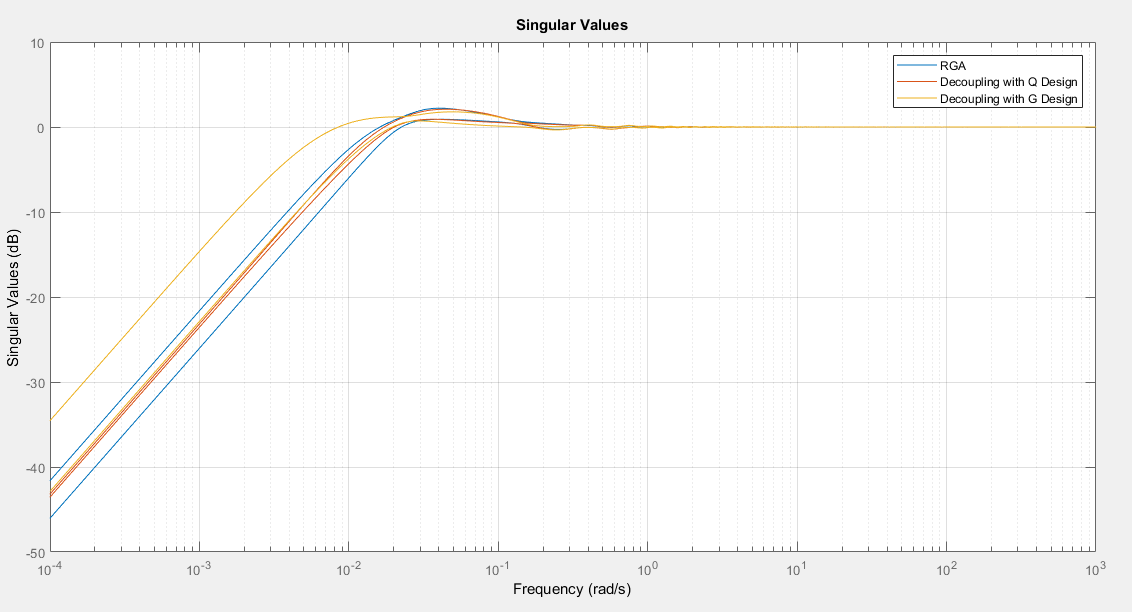
\includegraphics[width=0.9\textwidth]{./Graphics/SVD_MATLAB.png}
\caption{Robusteness of the MIMO}
\label{c:robustness:f:mimo_svd}
\end{minipage}
\end{figure}

%!TEX root = ../studentischeArbeiten.tex
\chapter{Application to Physical Process Models}
\label{c:physical}

\section{Process Description and Problem Statement} \label{c:physical:s:process}

The aim of enginnering thermodynamics is - as stated earlier in Chap. \ref{c:intro} - to understand and optimize the  behaviour of technical systems used for energy transformation and transportation. Hence, a connection to the field of optimal control is a logical extension to maximize the efficiency. As described in sec. \ref{c:thermo:s:process} the systems states are general interconnected by both physical components and physical phenomena. In the following section the coupling due to physical phenomena will be investigated.\\

The process at hand is an anticlockwise refrigeration process, shown in Fig.\ref{c:physical:f:model} in technical schematics and in Fig.\ref{c:physical:f:ph} in the pressure-specific enthalpy diagram. The model used for simulation in the scope of this work was provided and consists of a simple valve, according to Eq.\ref{c:thermo:e:throttle}, heat exchanger model fitted to experimentation data and a compressor modeled with a linear efficiency.\\

\begin{minipage}[c]{0.45\textwidth}
\includesvg[width = \textwidth]{Graphics/model_cycle}
\caption{Refrigeration cycle, component view}
\label{c:physical:f:model}
\end{minipage}%
\hspace{0.05\textwidth}%
\begin{minipage}[c]{0.45\textwidth}
\includesvg[width = \textwidth]{Graphics/ph_cycle}
\caption{Pressure over specific enthalpy diagram of the refrigeration cycle. }
\label{c:physical:f:ph}
\end{minipage}

Starting at the inlet of the compressor, Point 1, mechanical energy is given into the refrigerant increasing pressure and specific enthalpy in an isentropic process. Then, energy is subtracted isobaric in form of heat between the point 2 and 3 via a heat exchanger, called gascooler. Afterwards, the pressure drops to via a throttle valve from point 3 to point 4 isothermal, where it reaches a settling tank. There, the fluid phase is separated from the gas phase. The purely gas phase is transported to the inlet of the compressor via another isothermal throttle between point 7 and 1. The pressure of the liquid phase is also reduced via a throttle between point 5 and 6, before another heat exchanger adds energy isobaric to the system.\\

The problem description from a control perspective involves the control of five variables, the high pressure, medium pressure, the overheating and undercooling. In the scope of this work, the control of high pressure and undercooling is investigated.This is conducted via the revolutions of the fan to control the difference in temperature between point 2 and 3 and the effective area of the valve, which controls the pressure drop between point 3 and 4.\\

At first, the theoretical properties of the individual parts are investigated. The process can be divided in three basic processes:
\begin{itemize}
\item Isobaric process with heat supply
\item Adiabatic isenthalpic process 
\item Isentropic process with exchange of (mechanical) work
\end{itemize}
These processes can be characterized using the First Law of Thermodynamics in differential form, see e.g. \cite[p.25]{Weigand2013}:

\begin{align}
\begin{split}
du &= d \left( h - pv \right ) \\ &= dh - v dp - p dv \\
&= \delta q + \delta w_{diss} - p dv
\end{split}
\label{c:thermo:e:firstlaw}
\end{align}
\nomenclature{$u$}{Specific Inner Energy}
\nomenclature{$h$}{Specific Enthalpy}
\nomenclature{$p$}{Pressure}
\nomenclature{$v$}{Specific Volume}
\nomenclature{$q$}{Specific Heat}
\nomenclature{$w$}{Specific Work}

Which states that the change in inner energy $u \in \mathbb{R}$ is equal to the sum of heat $\delta Q \in \mathbb{R}$ and dissipated work $\delta w_{diss} \in \mathbb{R}$ minus the pressure-volume work, depending on the pressure $p \in \mathbb{R}^+$ times the change in specific volume $v \in \mathbb{R}^+$. The internal energy can be related to the specific enthalpy $h = u +pv \in \mathbb{R}$.\\

The Second Law of Thermodynamics as formulated by Gibbs \cite[p.59]{Struchtrup2014} is given by:

\begin{align}
\begin{split}
T ds &= du + p dv \\
 &= d( h - pv ) + p dv \\
 &= dh - vdp
\end{split}
\label{c:thermo:e:secondlaw}
\end{align}
\nomenclature{$T$}{Temperature}
\nomenclature{$s$}{Specific Enthropy}

Defining two independent to be state variables the specific volume $v$ and temperature $T$ and substitute Eq.\ref{c:thermo:e:firstlaw} in Eq.\ref{c:thermo:e:secondlaw}:

\begin{align}
\begin{split}
T ds &= du + p dv \\
&= \delta q  + \delta w_{diss}
\end{split}
\label{c:thermo:e:firstandsecondlaw}
\end{align}

Since the total differential of the inner energy is given by


\begin{align}
\begin{split}
du &= \left( \frac{du}{dT} \right)_v dT  + \left( \frac{du}{dv} \right)_T dv
\end{split}
\label{c:thermo:e:innerenergydiff}
\end{align}

Substitute Eq. \ref{c:thermo:e:innerenergydiff} in \ref{c:thermo:e:firstandsecondlaw} while using the definition for the specific heat capacity at constant volume $c_V = \left(\frac{\partial u}{\partial T}\right)_v \in \mathbb{R}^+$ holds:

\begin{align*}
\begin{split}
T ds &= \left( \frac{\partial u}{\partial T} \right)_v dT  + \left( \frac{\partial u}{ \partial v} \right)_T dv + p dv \\
&= c_v dT + \left[ p + \left( \frac{\partial u}{\partial v}\right)_T\right] dv
\end{split}
\end{align*}

Using the relation \cite[p.375]{Struchtrup2014} $T\left( \frac{\partial s}{\partial v}\right)_T = \left( \frac{\partial u}{\partial v}\right)_T + p $ and the Maxwell Relation $\left( \frac{\partial s}{\partial v}\right)_T = \left( \frac{\partial p}{\partial T}\right)_v = \frac{\beta}{\kappa} $ the equation becomes:

\begin{align}
\begin{split}
T ds &= \left( \frac{\partial u}{\partial T} \right)_v dT  + \left( \frac{\partial u}{ \partial v} \right)_T dv + p dv \\
\delta q &= c_v dT + T \frac{\beta}{\kappa} dv
\end{split}
\label{c:thermo:e:isobaricHeat}
\end{align}
\nomenclature{$c_v$}{Specific Heat Capacity at Constant Volume}
\nomenclature{$\beta$}{Coefficient of Thermal Expansion at Constant Pressure}
\nomenclature{$\kappa$}{Coefficient of Compressibility}

The coefficient of thermal expansion at constant pressure $\beta \in \mathbb{R}$ is defined by $\frac{1}{v}\left( \frac{dv}{dT} \right)_p = \beta$ and the compressibility $\kappa = \left( \frac{\partial v}{\partial p} \right)_T \in \mathbb{R}^+$ substitute the differential change of pressure due to temperature at constant volume via the chain rule.\newline

Eq. \ref{c:thermo:e:isobaricHeat} states that the exchange of heat in the isobaric process results in a change of specific volume and temperature. \\

The massflow $\frac{dm}{dt} = \dot{m} \in \mathbb{R}$ from A to B through a throttle can be described by a function of the density $\rho = \frac{1}{v} \in \mathbb{R}^+$, the effective area $A_{eff} \in \mathbb{R}^+$ and the difference in pressure 

\begin{align}
\begin{split}
\dot{m} & = A_{eff} \sqrt{2 \rho_A  \left( p_A -p_B \right) }
\end{split}
\label{c:thermo:e:throttle}
\end{align}
\nomenclature{$A_{eff}$}{Effective Area}
\nomenclature{$\rho$}{Density , Specific Mass}
\nomenclature{$\dot{m}$}{Massflow}

which directly relates the difference pressure $p_A - p_B = \Delta p > 0$ to the exchange of heat. Assume a constant mass flow, a constant effective Area and a constant pressure niveau $p_B$ due to perfect controller of the system, the energetic coupling between fan and pressure can be seen. If heat is added before A as described by Eq. \ref{c:thermo:e:isobaricHeat} the Temperature in A will be influenced as well the pressure due to the change in the specific volume and therefore the density via Eq.\ref{c:thermo:e:throttle}.\\

The isenthalpic, adiabat throttling process can be described by the Joule-Thomson Coefficient \cite[p.387]{Struchtrup2014}. The equation relates the change in temperature and pressure to each other via

\begin{align}
\begin{split}
\left( \frac{\partial T}{\partial p}\right)_h &= -\frac{1}{c_p} \left(\frac{\partial h}{ \partial p} \right)_T \\
&= \frac{v}{c_p}\left( T\beta - 1 \right) 
\end{split}
\label{c:thermo:e:joulethomson}
\end{align}

Where $c_p = \left(\frac{\partial h}{\partial T} \right)_p \in \mathbb{R}^+$ is the specific heat at constant pressure which relates the change in entropy due to a change in temperature.
Eq. \ref{c:thermo:e:joulethomson} and Eq. \ref{c:thermo:e:throttle} relate the change in pressure via variation of the effective Area to the change in temperature. \\

Eq. \ref{c:thermo:e:isobaricHeat}, \ref{c:thermo:e:throttle} and \ref{c:thermo:e:joulethomson} show the thermodynamic coupling of the system. They are highly nonlinear and give an ideal coupling for the quasi stationary processes and the choosen states pressure and temperature. Since both couplings take effect at the same time, a reasonable estimation of the process trajectory is difficult. \\

An important fact is that none of the equations above depend explicitly on the time. Rather,all coefficients above are functions of the thermodynamic states $p,v,T,s$ which are depending on time. Assuming quasi stationary behavior of the system for every coefficient $c \in \left\lbrace \beta, \kappa, c_v, c_p \right\rbrace$ can be related to the static gain of the couplings.\\

\section{Identification of the FOTD model} \label{c:physical:s:identification}

In the following section, the identification process is laid out and investigated within the simulation model. At first, some basics of the behavior shall be discussed. In Sec.\ref{c:physical:s:process} the thermodynamic properties of the gain has been investigated. The relations established before can be qualitatively extended to the whole technical system including the valve and the fan.\\

To estimate the effects of a change in input, the energy of Point 3 is evaluated. Assuming that the initial change in input result in a change of the internal energy at the outlet of the gascooler, the energy conservation can be formulated as:

\begin{align*}
\begin{split}
\int \left(\dot{m} c_p T_3 + \frac{\dot{m}}{\rho} p_3 \right) dt &=
\int \left(\dot{m} c_p T_{3'} + \frac{\dot{m}}{\rho} p_{3'} \right) dt \\
\rho c_p\left(T_{3} - T_{3'}\right)  + p_{3} - p_{3'} &= 0 \\
\rho c_p \Delta T_u + \Delta p_u &= 0
\end{split}
\end{align*}

From which can be concluded that the pressure and temperature change due to an external input $\Delta p_u, \Delta T_u \in \mathbb{R}$ are of opposite sign. \\

Increasing the revolution speed of a fan will increase the amount of heat transported out of the systems boundaries. Hence, the gain will be negative, since the temperature will decrease. If the temperature will decrease $\Delta T_u > 0$ and therefore the pressure at Point 3 will decrease to ensure that the energy of the system is conserved by $\Delta p_u < 0$.\\

Likewise, if the effective area of the throttle is increased, the pressure at the outlet of the gascooler will decrease, meaning $\Delta p_u > 0$. Hence, $\Delta T_u < 0$, meaning that the temperature after the excitation of the valve must be greater than before.\\

\begin{figure}[H]
\includesvg[width = \textwidth]{Graphics/ph_cycle_2}
\caption{Pressure over specific enthalpy diagram of the refrigeration cycle, Effects of an increase in $A_{eff}$ (blue) and $n$ (green) }
\label{c:physical:f:ph2}
\end{figure}

This is illustrated in Fig.\ref{c:physical:f:ph2}, where both processes are given qualitatively. In terms of the steady state gain of the transfer function matrix, this can be written as:

\begin{align*}
sign\left(\ma{G}_0 \right)
= \begin{bmatrix}
-1 & +1 \\
-1 & -1 
\end{bmatrix}
\end{align*}

This effect can be seen in Fig. \ref{c:physical:f:identification_example}, where a simulation of the system with an identification has been performed. Both the rotational speed of the fan and the effective area have been decreased to avoid crossing the saturated liquid line. The full line shows the impact of a change in the effective area on both the pressure and the temperature while the dashed line represents the influence of a change in the rotational speed of the fan. The identification has been performed at a ambient temperature $T_{amb} = 295 K $ with a heat of $\dot{Q}_{In} = -60 kW$ applied to the system. This results at an optimal working point of $\left( p_2, T_2 \right) = \left( 76.60 bar , 298.00 K\right)$ which is calculated using an formula based on optimization studies.

\begin{figure}[H]
\includesvg[width = \textwidth]{Graphics/Identification_Example_Physical}
\caption{Example of the influence of scaled input steps within the simulation model}
\label{c:physical:f:identification_example}
\end{figure}

It can be seen that the system is monotonic increasing and shows a very similar behavior to a higher order system. The system is identified using the area approach described in Ch.\ref{c:identification}. The transfer function matrix consisting of FOTD models is given by :

\begin{align*}
\ma{\hat{G}} = \begin{bmatrix}
\frac{-2.363}{45.943s+1}e^{-17.381s} & 
\frac{7.236}{49.723s+1}e^{-14.230s} \\
\frac{-3.177}{26.225s+1}e^{-15.645s} &
\frac{-4.399}{72.381s+1}e^{-7.953s}
\end{bmatrix}
\end{align*}

However, these results can vary depending on the operating conditions, e.g. ambient temperature, the systems state, e.g. pressure and temperature at the outlet of the gascooler, and the parameter like piping length, compressor model etc.. Parameter studies have been performed to estimate the effect of dominant parameters of the system, e.g. the valve dynamics, fan dynamics and number of tubes of the heat exchanger. The evaluation of all results of this study would go beyond the scope of this work, but for reasons of completeness the influence of the cooling capacity and the ambient temperature on the FOTD parameter is shown in Fig. \ref{c:physical:f:parameter_variation}.

\begin{figure}[H]
\includesvg[width = \textwidth]{Graphics/FOTD_Change}
\caption{Variation of the FOTD model parameter due to simulation parameter and operating conditions}
\label{c:physical:f:parameter_variation}
\end{figure}

It can be noticed that while the gain of the transfer functions connected to the fan are sensitive to changes in the model parameter, the gain of transfer functions related to the valve are only different in an offset. $K_{11}$, the gain of the fan to the temperature, is decreasing over the ambient temperature. If the temperature difference between point 2 and 3 is large, smaller changes will occur because most of the heat is already transported out of the system. If the difference is small, large variations of the rotational speed will significantly increase the heat transported out of the system. Therefore the gain is large at lower ambient temperatures which correspond to lower pressure levels, where the distance between isotherms is large. The same reasoning can be used to explain the decrease of the gain from fan to pressure $K_{21}$ where an appropriate scaling with the nonlinear material values has to be taken into account.\\

Likewise the transfer function gain $K_{22}$ is most likely depending on variations of the density and the mass flow through the valve, hence the nearly quadratic form and a variation given only by an offset. The same can be said for the gain $K_{12}$, also scaled with the nonlinear material values. An interesting property is given in form of the lags $T_{12},T_{21}$ which are identical for the marked example scenario. Hence, the time dependent behavior of the processes is most likely governed by its physical properties and not by the technical components. With the difference in delay, $L_{12} \geq L_{21}$, the assumption that the delay is strongly dependent on the mass flow and hence the fluid flow direction is obvious.\\

To estimate the error $\Delta_D \in \mathbb{C}$ of the simple decoupling, given in terms of Eq.\ref{c:controller:e:complexerror}, the steady state of the system is evaluated for all parameter values and shown in Fig.\ref{c:physical:f:complex_error}. It can be seen that the error is within a certain limits and does not exceed $0.68$. Also, all variations of the system show a similar behavior, only scaled for ambient temperatures $T_{amb}\geq 283 ~K$. Hence, it is most likely that the error is strongly dominated by the transfer functions connected to the valve. The error can be also used to indicate the usefulness of deriving a model for the combined transfer functions $g_{ii}^* = g_{ii}+ \sum_{j=1}^{n_y} \Sigma_{ji}g_{ij}$, which is obviously useful for higher ambient temperatures.

\begin{figure}[H]
\includesvg[width = \textwidth]{Graphics/Physical_ErrorSteadyState}
\caption{Error within the model use of the main diagonal within R2D2, steady state of the system}
\label{c:physical:f:complex_error}
\end{figure}

Likewise, the relative magnitude of the transfer functions, $\ma{E} \in \mathbb{C}^{n_y \times n_y}$ as given in Eq.\ref{c:controller:e:InteractionMagnitude}, can be calculated. Fig.\ref{c:physical:f:relative_mag} shows the determinant of the relative magnitudes for the decentralized controller and the added simple decoupler, which indicates the usefulness with respect to tracking behavior even though an error is dynamics is given.

\begin{figure}[H]
\includesvg[width = \textwidth]{Graphics/Physical_Dominance_SteadyState}
\caption{Relative magnitude within the model for decentralized control (full) and simple decoupling (dashed), steady state of the system}
\label{c:physical:f:relative_mag}
\end{figure}

It is also important to notice that while in theory only the physical effects are measured, in practice effects of all other controllers will be measured and taken into account. Hence, not only the influence of the valve to the temperature of point 2 is measured but the effect of the valve on point 2 and all closed loops of the system, meaning the loops for controlling points $(1,3,4,5,6,7)$.\\


\newpage
\section{Closed Loop Results} \label{c:physical:s:closedloop}

In the following section, some results of the autotuning methods are shown. The simulation has used a very robust controller to derive a steady state, where the controller was switched of and the experiment for identification has been performed. Afterwards, the model with the calculated controller parameters has been started and evaluated with respect to disturbance rejection and tracking performance. A static decoupled system is not explicitly given, since the simulation was not been able to start in all cases with the controller at hand.\\

Three cases are presented and the closed loop behavior with respect to tracking performance and disturbance rejection is shown. At first, the identification example as shown in Fig.\ref{c:physical:f:identification_example} is examined. The process operates with $T_{amb} = 290 K,~Q_C = -50 kW$. In Fig.\ref{c:physical:f:disturbance1} an input disturbance is simulated with a scaled step function acting on the effective Area at $6000~s$ and likewise at $10000~s$ for the rotational speed.

\begin{figure}[H]
\includesvg[width = \textwidth]{Graphics/DisturbanceExample_Physical}
\caption{Disturbance rejection of the closed loop simulated by a step acting on the systems input, Example 1}
\label{c:physical:f:disturbance1}
\end{figure}

It can be seen that both temperature and pressure act immediately on the disturbance. However, the controller enhanced by a simple decoupling method is able to return to the set point much faster than its purely decentralized counterpart. This is an indicator for the effect of the interconnections in the system, since the disturbance signal is able to spread out over all loops and hence last longer in the control loop if no compensation in form of the splitter is given.\\

Additionally, the overshoot due to the rejections is decreased, which can be related to the interconnections as well, since any error acts on every output for a purely decentralized control.\\

In Fig.\ref{c:physical:f:tracking1} the set point of pressure has been changed at $6000~s$ by a unit step, so is the set point of the temperature at $10000~s$. The effects due to interaction are visible immediately, since the temperature is influenced by the excitation of the valve. Due to the coupling of the loops, this resembles in an overshoot of the pressure. Likewise the set point change in temperature acts on the pressure, where the effects are also minimized due to the splitter.

\begin{figure}[H]
\includesvg[width = \textwidth]{Graphics/TrackingExample_Physical}
\caption{Tracking behavior of the closed loop simulated by a step acting on the systems set point, Example 1}
\label{c:physical:f:tracking1}
\end{figure}

Next, both ambient temperature and cooling capacity have been changed to 
$T_{amb} = 295 K,~Q_C = -60 kW$. The disturbance rejection is shown in Fig.\ref{c:physical:f:disturbance2}, the tracking performance in Fig.\ref{c:physical:f:tracking2}. Both scenarios show similar behavior by reducing both settling time and magnitude of the interaction while performing better with respect to tracking behavior.

\begin{figure}[H]
\includesvg[width = \textwidth]{Graphics/DisturbanceExample_Physical2}
\caption{Disturbance rejection of the closed loop simulated by a step acting on the systems input, Example 2}
\label{c:physical:f:disturbance2}
\end{figure}

It is worth noticing that the coupling between the valve and temperature has nearly canceled out, as can be seen in Fig.\ref{c:physical:f:tracking2}. This indicates a strong similarity between both processes with respect to its dynamics. Likewise, the strong interconnection between the fan and the pressure is weakened by the use of a splitter.

\begin{figure}[H]
\includesvg[width = \textwidth]{Graphics/TrackingExample_Physical2}
\caption{Tracking behavior of the closed loop simulated by a step acting on the systems set point, Example 2}
\label{c:physical:f:tracking2}
\end{figure}

The last example is operated at $T_{amb} = 272 K,~Q_C = -65 kW$. Again, the use of a splitter minimizes the distribution of disturbances throughout the closed loop system, as can be seen in Fig.\ref{c:physical:f:disturbance3}. While the settling time is not enhanced significant, the overshoot due to a disturbance in the rotational speed is compensated quicker.\\

The tracking behavior of the process is shown in Fig.\ref{c:physical:f:tracking3}. The benefits of the splitter with respect to set point change are clearly visible, since both disturbances due to interconnections can be minimized while keeping the performance of the decentralized control.\\

\begin{figure}[H]
\includesvg[width = \textwidth]{Graphics/DisturbanceExample_Physical3}
\caption{Disturbance rejection of the closed loop simulated by a step acting on the systems input, Example 3}
\label{c:physical:f:disturbance3}
\end{figure}


From the examples given above, the nonlinearity of the system is clearly visible in the performance of the closed loop and the splitter. While not being always useful with respect to disturbance rejection, the compensation of the signals never amplifies the unwanted behavior. Instead in almost all cases the tracking performance is enhanced while the disturbance rejection is at least as good as given by the not compensated controller.\\

\section{Review}\label{c:physical:s:review}

This chapter has given some important insights to the system and the behavior of the applied identification process. The FOTD model of all transfer functions is shown to be sensitive to change in physical parameter and operational conditions.

\begin{figure}[H]
\includesvg[width = \textwidth]{Graphics/TrackingExample_Physical3}
\caption{Tracking behavior of the closed loop simulated by a step acting on the systems set point, Example 3}
\label{c:physical:f:tracking3}
\end{figure}

However, over all changes a similar behavior with respect to the ambient temperature is visible. The two major remarks with respect to the change in behavior and interconnection are visible in the gain of valve related transfer functions and the time constants of the cross couplings. Both $K_{12}$ and $K_{22}$ show only two characteristic curves over the ambient temperature, which indicates a dominant parameter for both curves. Likewise, the lag of the interconnections is equal while the delay differs strongly. As mentioned, this can most likely be related to the fluids physical properties and its flow direction.\\

The examples given in Sec.\ref{c:physical:s:closedloop} show the benefits of the usage of a compensation of unwanted effects by applying the splitter. The behavior of all processes with respect to disturbance rejection have been at least as bad as the purely decentralized controller but mostly better. The tracking performance is enhanced in all cases, even though the error in the transfer function, shown in Fig.\ref{c:physical:f:complex_error}, is quite large.\\

\chapter{Conclusion and Outlook}
\label{c:conclusion}

%\chapter{Grundlagen}
\label{sec:Grundlagen}



\section{Wert und Einheit}
\label{sec:Unit}
Viele Einheiten lassen sich sch�ner darstellen mit dem Latex Befehl \verb|\unit[]{}| beziehungsweise \verb|\unitfrac[]{}{}|. Siehe den Vergleich: ohne 1~m oder mit \unit[1]{m} bzw. ohne 1~m/sec oder mit \unitfrac[1]{m}{sec}. Des weiteren kann zum Beispiel mit \verb|\textcelsius| ein \textcelsius{} Symbol eingef�gt werden.

\section{�berschrift}
\label{sec:Quelltext}
Text Text Text Text Text Text Text Text Text Text Text Text Text Text Text Text Text Text Text Text Text Text Text Text Text Text Text Text Text Text Text Text Text Text Text Text Text Text Text Text Text Text Text Text Text Text Text Text Text Text Text Text Text Text Text Text Text Text Text Text Text Text Text Text Text Text Text Text Text Text Text Text

\section{Abbildungen einbinden}
\label{sec:pictures}
Text Text Text Text Text Text Text Text Text Text Text Text Text Text Text Text Text Text Text Text Text Text Text Text Text Text Text Text Text Text Text Text Text Text Text Text Text Text Text Text Text Text Text Text Text Text Text Text Text Text Text Text Text Text Text Text Text Text Text Text Text Text Text Text Text Text Text Text Text Text Text Text Text Text Text Text Text Text 


\begin{figure}[htbp]
  \centering
  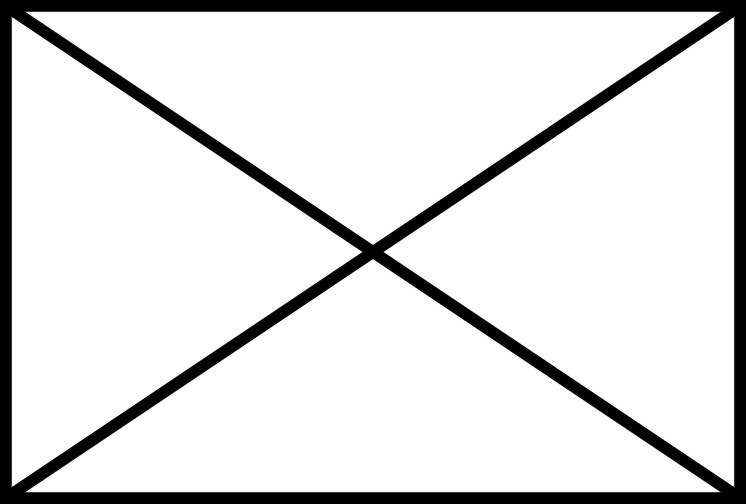
\includegraphics{pictures/empty.jpg}
  \caption{Einzelne Abbildung}
  \label{fig:singlepicture}
\end{figure}


Text Text Text Text Text Text Text Text Text Text Text Text Text Text Text Text Text Text Text Text Text Text Text Text Text Text Text Text Text Text Text Text Text Text Text Text Text Text Text Text Text Text Text Text Text Text Text Text Text Text Text Text Text Text Text Text Text Text Text Text Text Text Text Text Text Text Text Text Text Text Text Text Text Text Text Text Text Text Text Text Text Text Text Text Text Text Text Text Text Text Text Text Text Text Text Text Text Text Text Text Text Text Text Text Text Text Text Text Text Text Text Text Text Text Text Text Text Text Text Text Text Text Text Text Text Text Text Text Text Text Text Text Text Text Text Text Text Text Text Text Text Text Text Text Text Text Text Text Text 



Text Text Text Text Text Text Text Text Text Text Text Text Text Text Text Text Text Text Text Text Text Text Text Text Text Text Text Text Text Text Text Text Text Text Text Text Text Text Text Text Text Text Text Text Text Text Text Text Text Text Text Text Text Text Text Text Text Text Text Text Text Text Text Text Text Text Text Text Text Text Text Text Text Text Text Text Text Text Text Text Text Text Text Text Text Text Text Text Text Text Text Text Text Text Text Text Text Text Text Text Text Text Text Text Text Text Text Text Text Text Text Text Text Text Text Text Text Text Text Text Text Text Text Text Text Text Text Text Text Text Text Text Text 
%\addchap{Symbolverzeichnis}
\label{Symbolverzeichnis}

\begin{tabbing}
\hspace*{3.5cm}                              \=  \hspace*{10.0cm}                     \= \kill
\textbf{Formelzeichen}                       \> \textbf{Bedeutung}                    \> \textbf{Einheit} \\
~\\
${I}$                                        \> Strom                                 \> A  \\
${i}$                                        \> Getriebe�bersetzung                   \> -  \\
${l}$                                        \> L�nge                                 \> m  \\
${M}$                                        \> Drehmoment                            \> N  \\
${m}$                                        \> Masse                                 \> Kg \\
${n}$                                        \> Drehzahl                              \> 1/sec \\
${R}$                                        \> Widerstand                            \> $\Omega$ \\
${t}$                                        \> Zeit                                  \> sec \\
${U}$                                        \> Spannung                              \> V \\
~\\
${\alpha}$                           		 \> Drehwinkel von Gelenk 1               \> rad \\
${\beta}$                           	 	 \> Drehwinkel von Gelenk 2               \> rad \\
${\Delta \varepsilon}$   				 	 \> Aufl�sung der Drehwinkelsensoren      \> rad/Imp. \\
${\varepsilon}$                      		 \> Drehwinkel allgemein                  \> rad \\
${\theta}$              					 \> Tr�gheitsmoment                       \> Kg$\cdot$m$^2$ \\
~\\
~\\
\textbf{Indizes}                             \> \textbf{Bedeutung} \\
~\\
${0}$                                        \> Leerlauf \\
${el}$                                       \> elektrischer Teil der Motoren \\
${mech}$                                     \> mechanischer Teil der Motoren \\
${G}$                                        \> Getriebe \\
${i, j}$                                	 \> Laufindex (1, 2, 3, ...) \\
${Ref}$                                      \> Referenzwert \\
${soll}$                                     \> Sollgr��e \\
\end{tabbing}

\bibliography{chapters/mendeley_masterarbeit} 

\Anhang
\section{Erster Anhang}
\label{sec:Anhang_1}
Ein Anhang.


\section{Zweiter Anhang}
\label{sec:Anhang_2}
Ein weiterer Anhang.



%--------------------------------------------------
%--------------Ende eigener Kapitel----------------cl
%--------------------------------------------------

\makebackpage[trisec]%[<plain/info/addressinfo>]
\end{document}
cl